\documentclass[]{report}
\usepackage{lmodern}
\usepackage{setspace}
\setstretch{1.5}
\usepackage{amssymb,amsmath}
\usepackage{ifxetex,ifluatex}
\usepackage{fixltx2e} % provides \textsubscript
\ifnum 0\ifxetex 1\fi\ifluatex 1\fi=0 % if pdftex
  \usepackage[T1]{fontenc}
  \usepackage[utf8]{inputenc}
\else % if luatex or xelatex
  \ifxetex
    \usepackage{mathspec}
  \else
    \usepackage{fontspec}
  \fi
  \defaultfontfeatures{Ligatures=TeX,Scale=MatchLowercase}
\fi
% use upquote if available, for straight quotes in verbatim environments
\IfFileExists{upquote.sty}{\usepackage{upquote}}{}
% use microtype if available
\IfFileExists{microtype.sty}{%
\usepackage{microtype}
\UseMicrotypeSet[protrusion]{basicmath} % disable protrusion for tt fonts
}{}
\usepackage[margin=1in]{geometry}
\usepackage{hyperref}
\hypersetup{unicode=true,
            pdfborder={0 0 0},
            breaklinks=true}
\urlstyle{same}  % don't use monospace font for urls
\usepackage{color}
\usepackage{fancyvrb}
\newcommand{\VerbBar}{|}
\newcommand{\VERB}{\Verb[commandchars=\\\{\}]}
\DefineVerbatimEnvironment{Highlighting}{Verbatim}{commandchars=\\\{\}}
% Add ',fontsize=\small' for more characters per line
\usepackage{framed}
\definecolor{shadecolor}{RGB}{248,248,248}
\newenvironment{Shaded}{\begin{snugshade}}{\end{snugshade}}
\newcommand{\KeywordTok}[1]{\textcolor[rgb]{0.13,0.29,0.53}{\textbf{#1}}}
\newcommand{\DataTypeTok}[1]{\textcolor[rgb]{0.13,0.29,0.53}{#1}}
\newcommand{\DecValTok}[1]{\textcolor[rgb]{0.00,0.00,0.81}{#1}}
\newcommand{\BaseNTok}[1]{\textcolor[rgb]{0.00,0.00,0.81}{#1}}
\newcommand{\FloatTok}[1]{\textcolor[rgb]{0.00,0.00,0.81}{#1}}
\newcommand{\ConstantTok}[1]{\textcolor[rgb]{0.00,0.00,0.00}{#1}}
\newcommand{\CharTok}[1]{\textcolor[rgb]{0.31,0.60,0.02}{#1}}
\newcommand{\SpecialCharTok}[1]{\textcolor[rgb]{0.00,0.00,0.00}{#1}}
\newcommand{\StringTok}[1]{\textcolor[rgb]{0.31,0.60,0.02}{#1}}
\newcommand{\VerbatimStringTok}[1]{\textcolor[rgb]{0.31,0.60,0.02}{#1}}
\newcommand{\SpecialStringTok}[1]{\textcolor[rgb]{0.31,0.60,0.02}{#1}}
\newcommand{\ImportTok}[1]{#1}
\newcommand{\CommentTok}[1]{\textcolor[rgb]{0.56,0.35,0.01}{\textit{#1}}}
\newcommand{\DocumentationTok}[1]{\textcolor[rgb]{0.56,0.35,0.01}{\textbf{\textit{#1}}}}
\newcommand{\AnnotationTok}[1]{\textcolor[rgb]{0.56,0.35,0.01}{\textbf{\textit{#1}}}}
\newcommand{\CommentVarTok}[1]{\textcolor[rgb]{0.56,0.35,0.01}{\textbf{\textit{#1}}}}
\newcommand{\OtherTok}[1]{\textcolor[rgb]{0.56,0.35,0.01}{#1}}
\newcommand{\FunctionTok}[1]{\textcolor[rgb]{0.00,0.00,0.00}{#1}}
\newcommand{\VariableTok}[1]{\textcolor[rgb]{0.00,0.00,0.00}{#1}}
\newcommand{\ControlFlowTok}[1]{\textcolor[rgb]{0.13,0.29,0.53}{\textbf{#1}}}
\newcommand{\OperatorTok}[1]{\textcolor[rgb]{0.81,0.36,0.00}{\textbf{#1}}}
\newcommand{\BuiltInTok}[1]{#1}
\newcommand{\ExtensionTok}[1]{#1}
\newcommand{\PreprocessorTok}[1]{\textcolor[rgb]{0.56,0.35,0.01}{\textit{#1}}}
\newcommand{\AttributeTok}[1]{\textcolor[rgb]{0.77,0.63,0.00}{#1}}
\newcommand{\RegionMarkerTok}[1]{#1}
\newcommand{\InformationTok}[1]{\textcolor[rgb]{0.56,0.35,0.01}{\textbf{\textit{#1}}}}
\newcommand{\WarningTok}[1]{\textcolor[rgb]{0.56,0.35,0.01}{\textbf{\textit{#1}}}}
\newcommand{\AlertTok}[1]{\textcolor[rgb]{0.94,0.16,0.16}{#1}}
\newcommand{\ErrorTok}[1]{\textcolor[rgb]{0.64,0.00,0.00}{\textbf{#1}}}
\newcommand{\NormalTok}[1]{#1}
\usepackage{graphicx,grffile}
\makeatletter
\def\maxwidth{\ifdim\Gin@nat@width>\linewidth\linewidth\else\Gin@nat@width\fi}
\def\maxheight{\ifdim\Gin@nat@height>\textheight\textheight\else\Gin@nat@height\fi}
\makeatother
% Scale images if necessary, so that they will not overflow the page
% margins by default, and it is still possible to overwrite the defaults
% using explicit options in \includegraphics[width, height, ...]{}
\setkeys{Gin}{width=\maxwidth,height=\maxheight,keepaspectratio}
\IfFileExists{parskip.sty}{%
\usepackage{parskip}
}{% else
\setlength{\parindent}{0pt}
\setlength{\parskip}{6pt plus 2pt minus 1pt}
}
\setlength{\emergencystretch}{3em}  % prevent overfull lines
\providecommand{\tightlist}{%
  \setlength{\itemsep}{0pt}\setlength{\parskip}{0pt}}
\setcounter{secnumdepth}{5}
% Redefines (sub)paragraphs to behave more like sections
\ifx\paragraph\undefined\else
\let\oldparagraph\paragraph
\renewcommand{\paragraph}[1]{\oldparagraph{#1}\mbox{}}
\fi
\ifx\subparagraph\undefined\else
\let\oldsubparagraph\subparagraph
\renewcommand{\subparagraph}[1]{\oldsubparagraph{#1}\mbox{}}
\fi

%%% Use protect on footnotes to avoid problems with footnotes in titles
\let\rmarkdownfootnote\footnote%
\def\footnote{\protect\rmarkdownfootnote}

%%% Change title format to be more compact
\usepackage{titling}

% Create subtitle command for use in maketitle
\newcommand{\subtitle}[1]{
  \posttitle{
    \begin{center}\large#1\end{center}
    }
}

\setlength{\droptitle}{-2em}

  \title{}
    \pretitle{\vspace{\droptitle}}
  \posttitle{}
    \author{}
    \preauthor{}\postauthor{}
    \date{}
    \predate{}\postdate{}
  
\usepackage{mdframed}
\usepackage[utf8]{inputenc}
\usepackage[francais]{babel} % use french to compile pdf
\usepackage{geometry} % use to modify the margins
\geometry{hmargin = 4cm, vmargin = 3cm}
\usepackage{hyperref}
\usepackage{cite}
\usepackage{tocloft}
\usepackage{float}
\floatplacement{figure}{H}
\newcommand*\rfrac[2]{{}^{#1}\!/_{#2}}

\begin{document}

\setstretch{1}

\begin{centering}

\begin{figure}


\includegraphics[width=3.0cm, height=6cm]{../image/technique-logo.jpg} 

\includegraphics[width=5.0cm, height=3.5cm]{../image/condorcet.jpg}

\includegraphics[width=3.7cm, height=7cm]{../image/UMONS-logo.jpg}
\includegraphics[width=1.6cm, height=3.5cm]{../image/ECONUM-logo.pdf}

\end{figure}

\textcolor{white}{.}

\vspace{2.0 cm}

\Huge

{\bf Rapport de stage}

\vspace{1 cm}

\huge 
{\bf Mise en place d'une application web surveillant la croissance des coraux en mésocosmes.}

\vspace{1 cm}

\Large

Jordan Benrezkallah

\vspace{2 cm}

\normalsize
Maître de stage : Philippe Grosjean

Encadrant de stage : Guyliann Engels

Promoteur : Aline Leonet et David Coornaert


\vspace{2.5 cm}

\normalsize
HEH - Campus technique -
Bloc 3 du cursus Bachelier en Biotechnique

Année académique 2018-2019

\end {centering}


\includegraphics[width=4cm, height=3.5cm]{../image/fede.jpg}

\newpage

\null
\newpage

\setstretch{1}

\begin{centering}

\begin{figure}


\includegraphics[width=3.0cm, height=6cm]{../image/technique-logo.jpg} 

\includegraphics[width=5.0cm, height=3.5cm]{../image/condorcet.jpg}

\includegraphics[width=3.7cm, height=7cm]{../image/UMONS-logo.jpg}
\includegraphics[width=1.6cm, height=3.5cm]{../image/ECONUM-logo.pdf}

\end{figure}

\textcolor{white}{.}

\vspace{2.0 cm}

\Huge

{\bf Rapport de stage}

\vspace{1 cm}

\huge 
{\bf Mise en place d'une application web surveillant la croissance des coraux en mésocosmes.}

\vspace{1 cm}

\Large

Jordan Benrezkallah

\vspace{2 cm}

\normalsize
Maître de stage : Philippe Grosjean

Encadrant de stage : Guyliann Engels

Promoteur : Aline Leonet et David Coornaert


\vspace{2.5 cm}

\normalsize
HEH - Campus technique -
Bloc 3 du cursus Bachelier en Biotechnique

Année académique 2018-2019

\end {centering}


\includegraphics[width=4cm, height=3.5cm]{../image/fede.jpg}

\newpage

\null

\textcolor{white}{.}

\Huge 
{\bf Remerciements} \vspace{1 cm}

\normalsize
Je remercie le professeur Philippe Grosjean qui m'a accueilli dans son
laboratoire afin d'effectuer ce stage et qui a permis la mise en oeuvre
de celui-ci.

Je voudrai également remercier les autres personnes du laboratoire
d'Écologie Numérique des Milieux Aquatiques. Tout d'abord, je remercie
Guyliann Engels qui m'a suivi depuis le début, qui a répondu aux
nombreuses questions que je pouvais avoir et qui m'a accueilli dans son
bureau. Je remercie Antoine, le technicien capable de maintenir les
mésocosmes, il m'a de nombreuses fois prit le temps de m'aider. Je
remercie également les mémorants, Madeleine et Rémy pour tous les
échanges instructifs que j'ai pu avoir avec eux lors de ce stage. Je
remercie aussi Nicolas pour les conseils qu'il m'a prodigués.

Un dernier remerciement revient à Raphaël qui a créé l'application sur
laquelle je me suis basé pour commencer la mienne. \vfill
\null
\newpage

\textcolor{white}{.}

\Huge 
{\bf Résumé} \vspace{1 cm}

\normalsize

Depuis plusieurs années, les scientifiques et le grand public
s'intéressent fortement aux effets du changement climatique sur les
écosystèmes. Les coraux forment des écosystèmes marins complexes parmi
les plus riches en biodiversité. Le service d'EcoNum étudie
l'écophysiologie des scléractiniaires.

Les objectifs de ce stage sont multiples. Dans un premier temps il
faudra acquérir des connaissances suffisantes du langage de
programmation R. Ensuite, développer des outils permettant le monitoring
des coraux. Des boutures de coraux devront être réalisées ainsi que des
relevés réguliers de leurs masses tout au long de ce stage.

Un tableur en ligne sera conçu et contiendra l'ensemble des données
relevées. À partir de cela, une application web mise en place génèrera
plusieurs onglets. Le premier est une visualisation dynamique de la
croissance des boutures, le second est un tableau intéractif qui permet
de trier par colonnes dans une plage donnée. Enfin, le dernier onglet
une aide est disponible.

\vspace{2 cm}

\Huge 
{\bf Summary} \vspace{1 cm}

\normalsize
For several years, scientists and the general public have been strongly
interested in the effects of climate change on ecosystems. Corals form
complex marine ecosystems that are among the richest in biodiversity.
The EcoNum department studies the ecophysiology of sclerotia.

The objectives of this internship are multiple. First of all, it will be
necessary to acquire sufficient knowledge of the R programming language.
Then, develop tools to monitor corals. Coral cuttings should be carried
out as well as regular surveys of their masses throughout this course.

A spreadsheet will be designed and will contain all the data collected.
From this, a web application set up will generate several tabs. The
first is a dynamic visualization of the growth of cuttings, the second
is an interactive table that allows you to sort by columns in a given
range. Finally, the last tab a help is available.

\null
\newpage

\setstretch{1.2}

\tableofcontents

\null
\newpage

\textcolor{white}{.}

\Huge 
{\bf Lexique} \vspace{1 cm}

\normalsize
Aragonite : minéral composé de carbonate de calcium.

Carbonate de calcium (CaCO\textsubscript{3}) : composant majeur du
calcaire et constituant principal des coquilles d'animaux marins et du
corail.

Cnidaire : groupe (embranchement) d'espèces animales spécifiques du
milieu aquatique.

Corail : animal de l'embranchement des Cnidaires.

EcoNum : Service d'Écologie Numérique des Milieux Aquatiques.

Symbiose : association biologique, durable et réciproquement profitable,
entre deux organismes vivants.

Monitoring : suveillance, contrôle.

Scléractiniaire : ordre principal des coraux durs.

Script : suite de commandes permettant d'automatiser une tâche.

\emph{Seriatopora hystrix} Dana 1846 : espèce de scléractiniaires.

UMons : université de Mons.

Zooxanthelle : algue unicellulaire pouvant vivre en symbiose avec le
corail.

\null
\newpage

\chapter{Présentation}\label{presentation}

\section{Présentation de
l'entreprise}\label{presentation-de-lentreprise}

Mon stage de fin d'études, se déroule à l'université de Mons dans le
service d'Écologie Numérique des Milieux Aquatiques (abrégé en EcoNum)
du département de Biologie.

L'Université de Mons (UMONS), est une université francophone implantée
en Belgique, dans la province du Hainaut. Elle est constituée de 2
écoles et de 7 facultés, dont la faculté des Sciences.

Le Département de biologie de la faculté des Sciences est impliqué dans
la formation des étudiants et dans la recherche.

Ce département comprend 5 services, dont le service d'Écologie Numérique
des Milieux Aquatiques. Ce dernier étudie le comportement des
écosystèmes aquatiques complexes, tels les communautés planctoniques et
les récifs coralliens, face aux changements de leur environnement.

Le Service développe également des outils en science des données, y
compris dans le domaine du data mining, des big data, et de la recherche
reproductible. Il participe à des études sur les logiciels Open Source.

Le laboratoire d'EcoNum est situé sur le campus de la plaine de Nimy (A)
(Fig. 1.1) dans le pentagone (1) (Fig. 1.2).

\begin{figure}
\centering
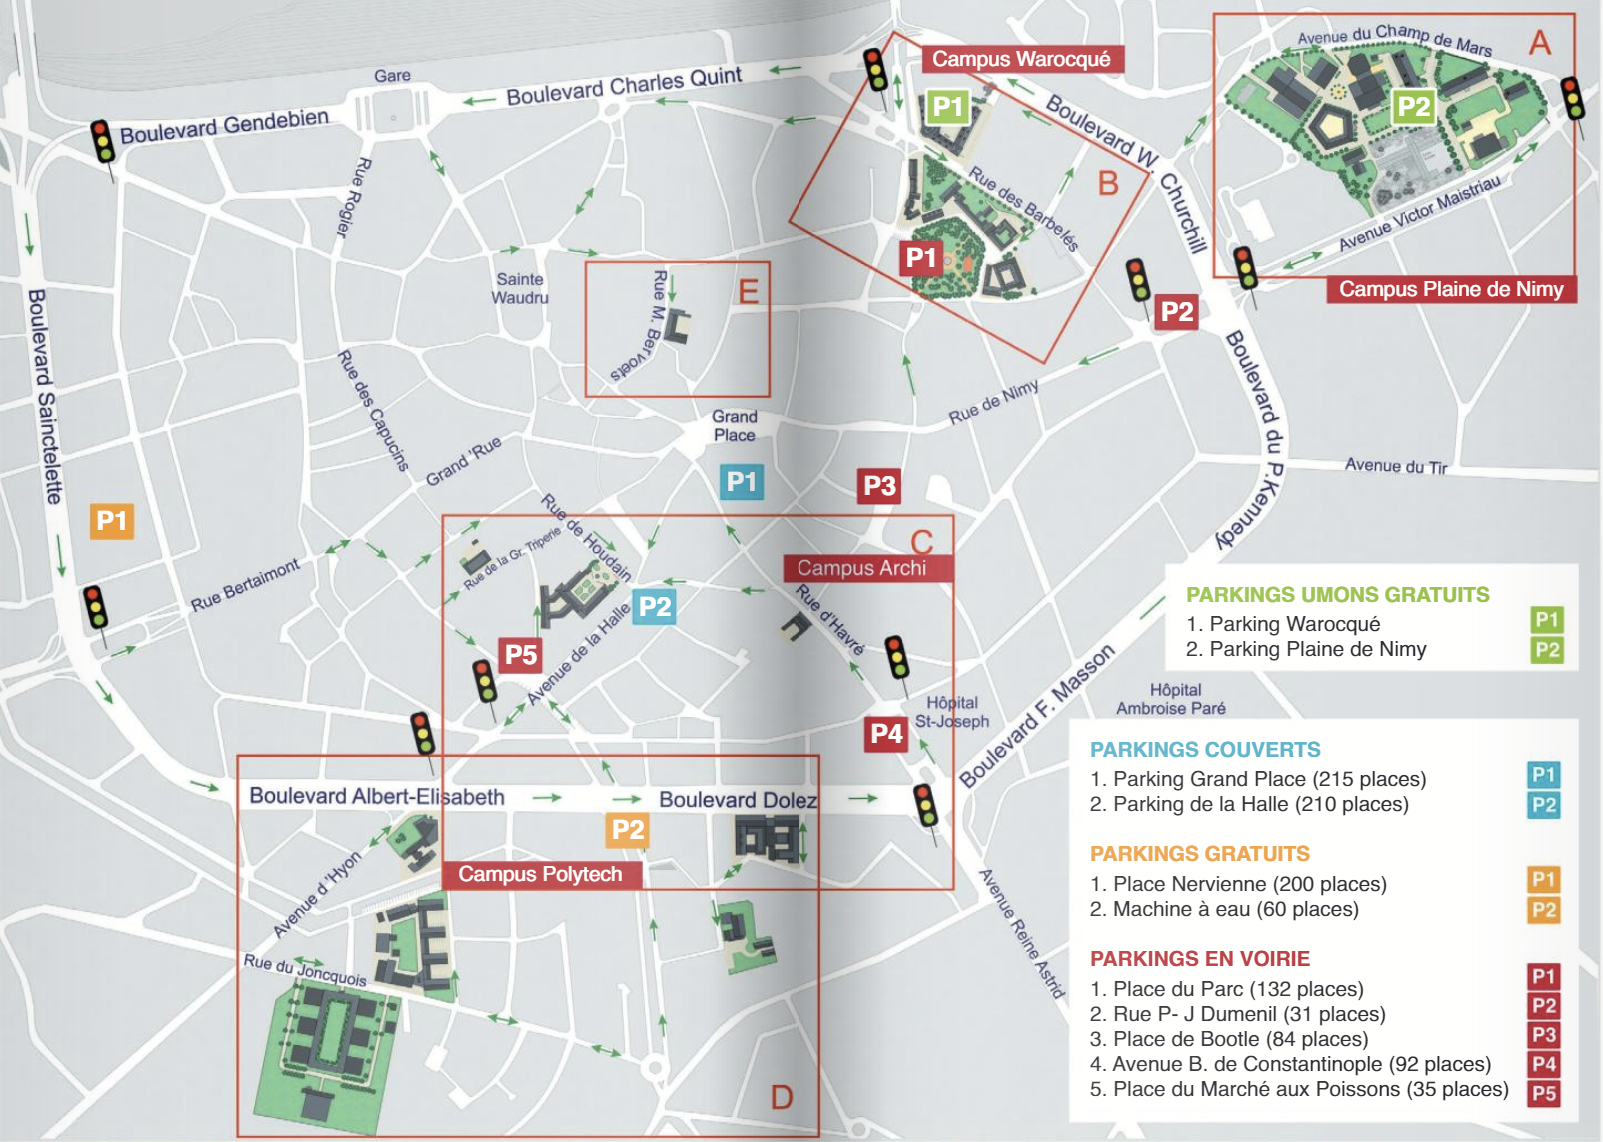
\includegraphics{../image/plan-campus.png}
\caption{Carte de la ville de Mons}
\end{figure}

\begin{figure}
\centering
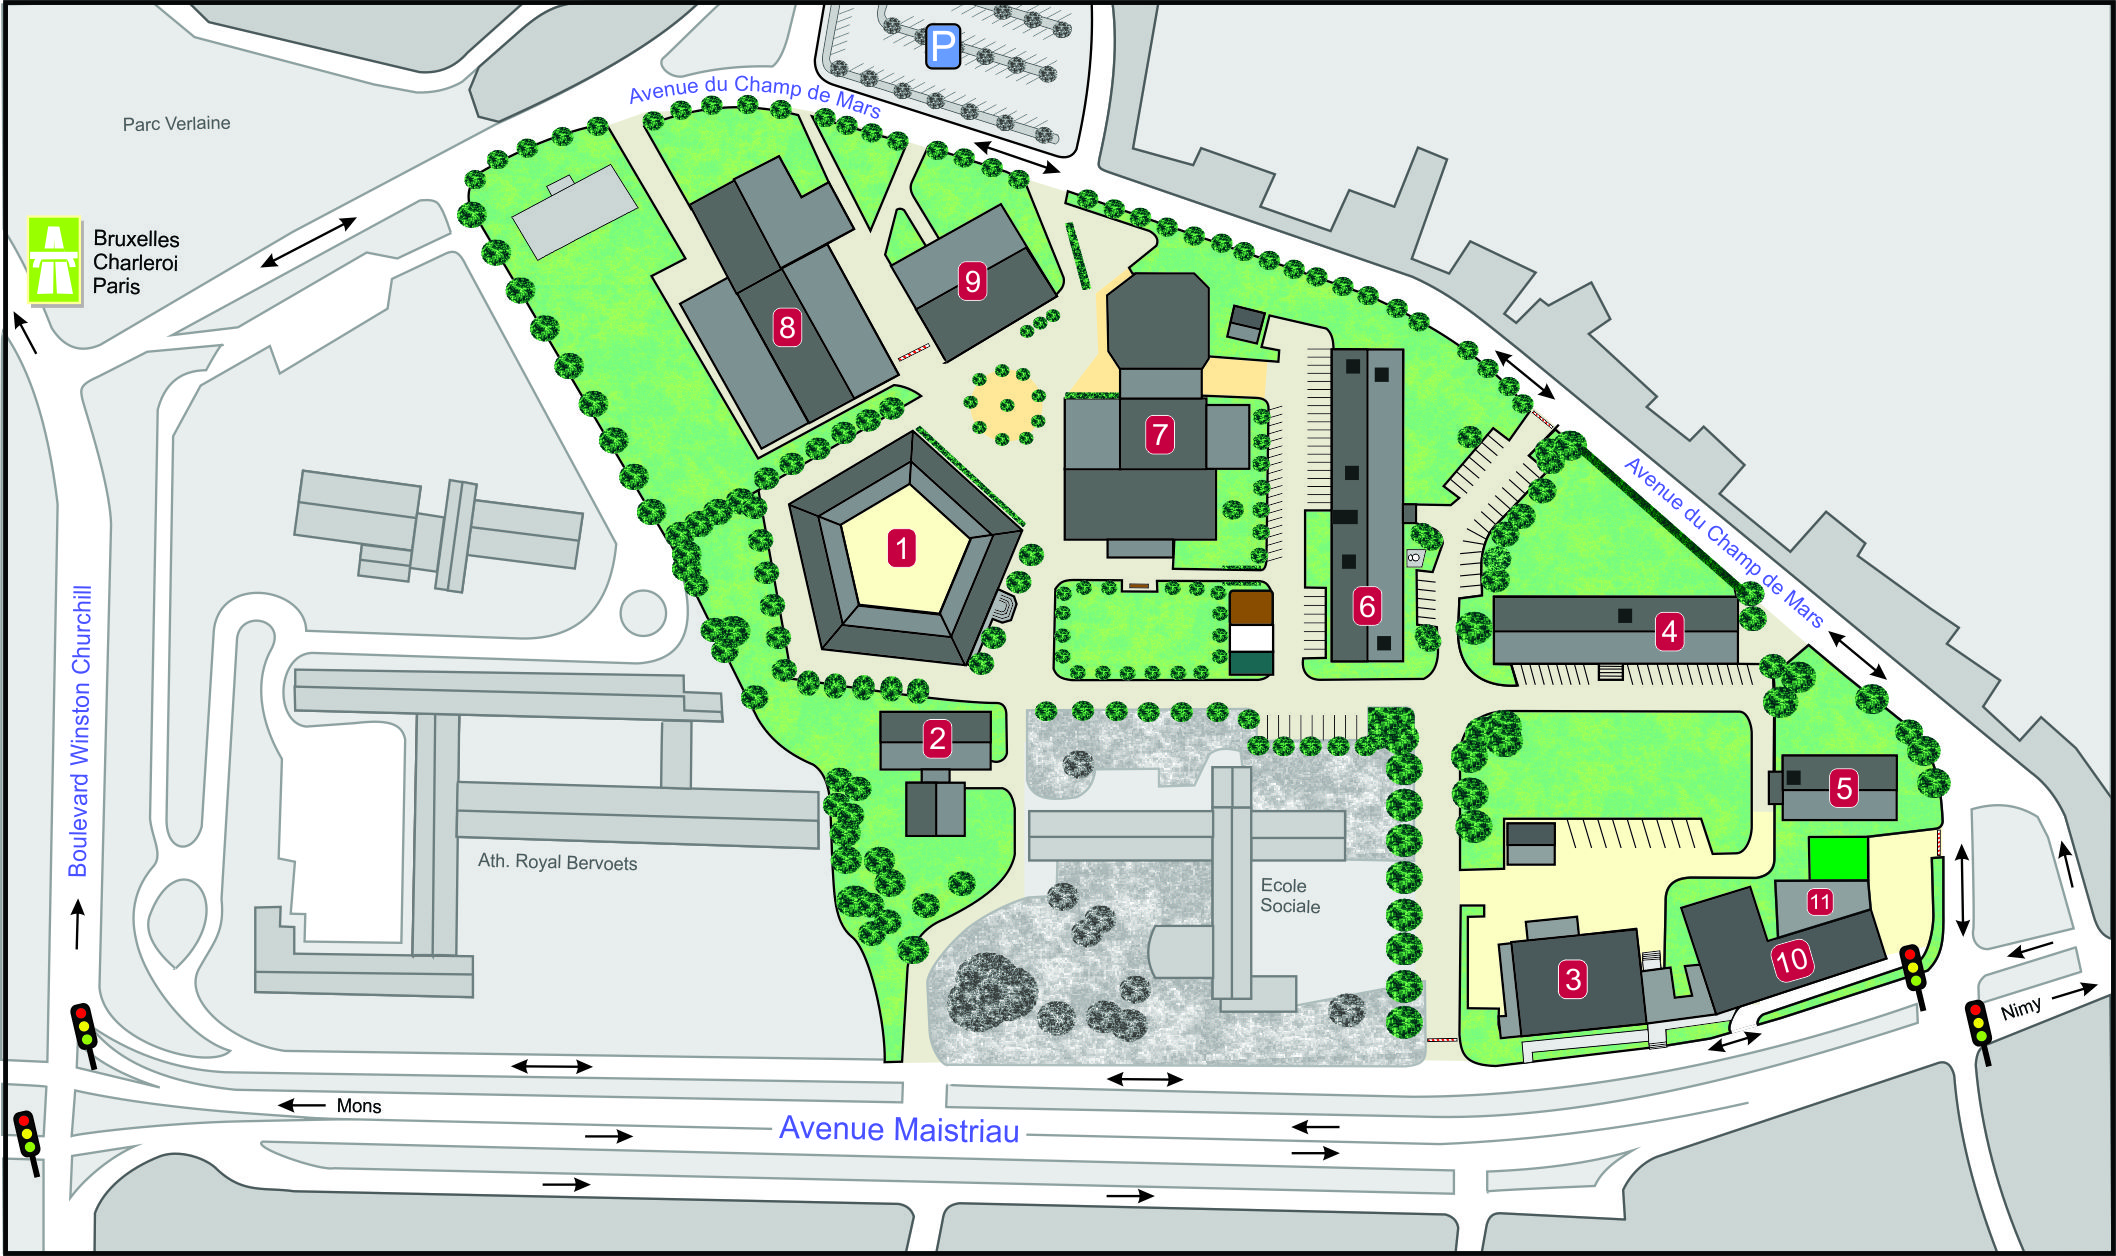
\includegraphics{../image/plaine-Nimy.jpg}
\caption{Carte du campus de la plaine de Nimy}
\end{figure}

\section{Présentation de l'équipe}\label{presentation-de-lequipe}

\subsection{Philippe Grosjean}\label{philippe-grosjean}


\includegraphics[width=4.00000cm]{../image/Grosjean2.jpg}

Mon maître de stage est Monsieur Philippe Grosjean. Il mène plusieurs
projets de recherches sur l'identification automatique du plancton par
des algorithmes de \emph{machine learning}, sur l'écophysiologie des
scléractiniaires et sur le développement de logiciel pour l'écologie.

Il enseigne également la science des données biologiques, l'écologie
marine, l'écophysiologie et l'océanographie générale aux étudiants en
biologie.

Il développe des outils Open Source comme la \emph{SciViews Box}, qui
est une machine virtuelle contenant une suite de logiciels préconfiguré
pour l'utilisation de ses étudiants et des chercheurs.

Il encadre 1 doctorant et 2 étudiants en masters.

\subsection{Guyliann Engels}\label{guyliann-engels}


\includegraphics[width=4.00000cm]{../image/Guyliann.jpg}

Guyliann Engels est chercheur et assistant au sein du service. Il
effectue sa thèse sur l'écophysiologie du corail, où il utilise un
mésocosme pour étudier les stress des coraux engendrés par la
modification de leurs nutriments essentiels (composés azotés et
phosphorés). Il utilise fréquemment les outils de statistiques R et
RStudio (avec R Markdown, R Notebook).

Il encadre mon travail.

\subsection{Antoine Batigny}\label{antoine-batigny}

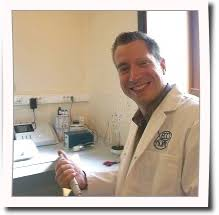
\includegraphics[width=4.00000cm]{../image/antoine2.jpg}

Antoine Batigny est le technicien du service. Il gère principalement les
mésocosmes.

\subsection{Rémy Dugauquier}\label{remy-dugauquier}

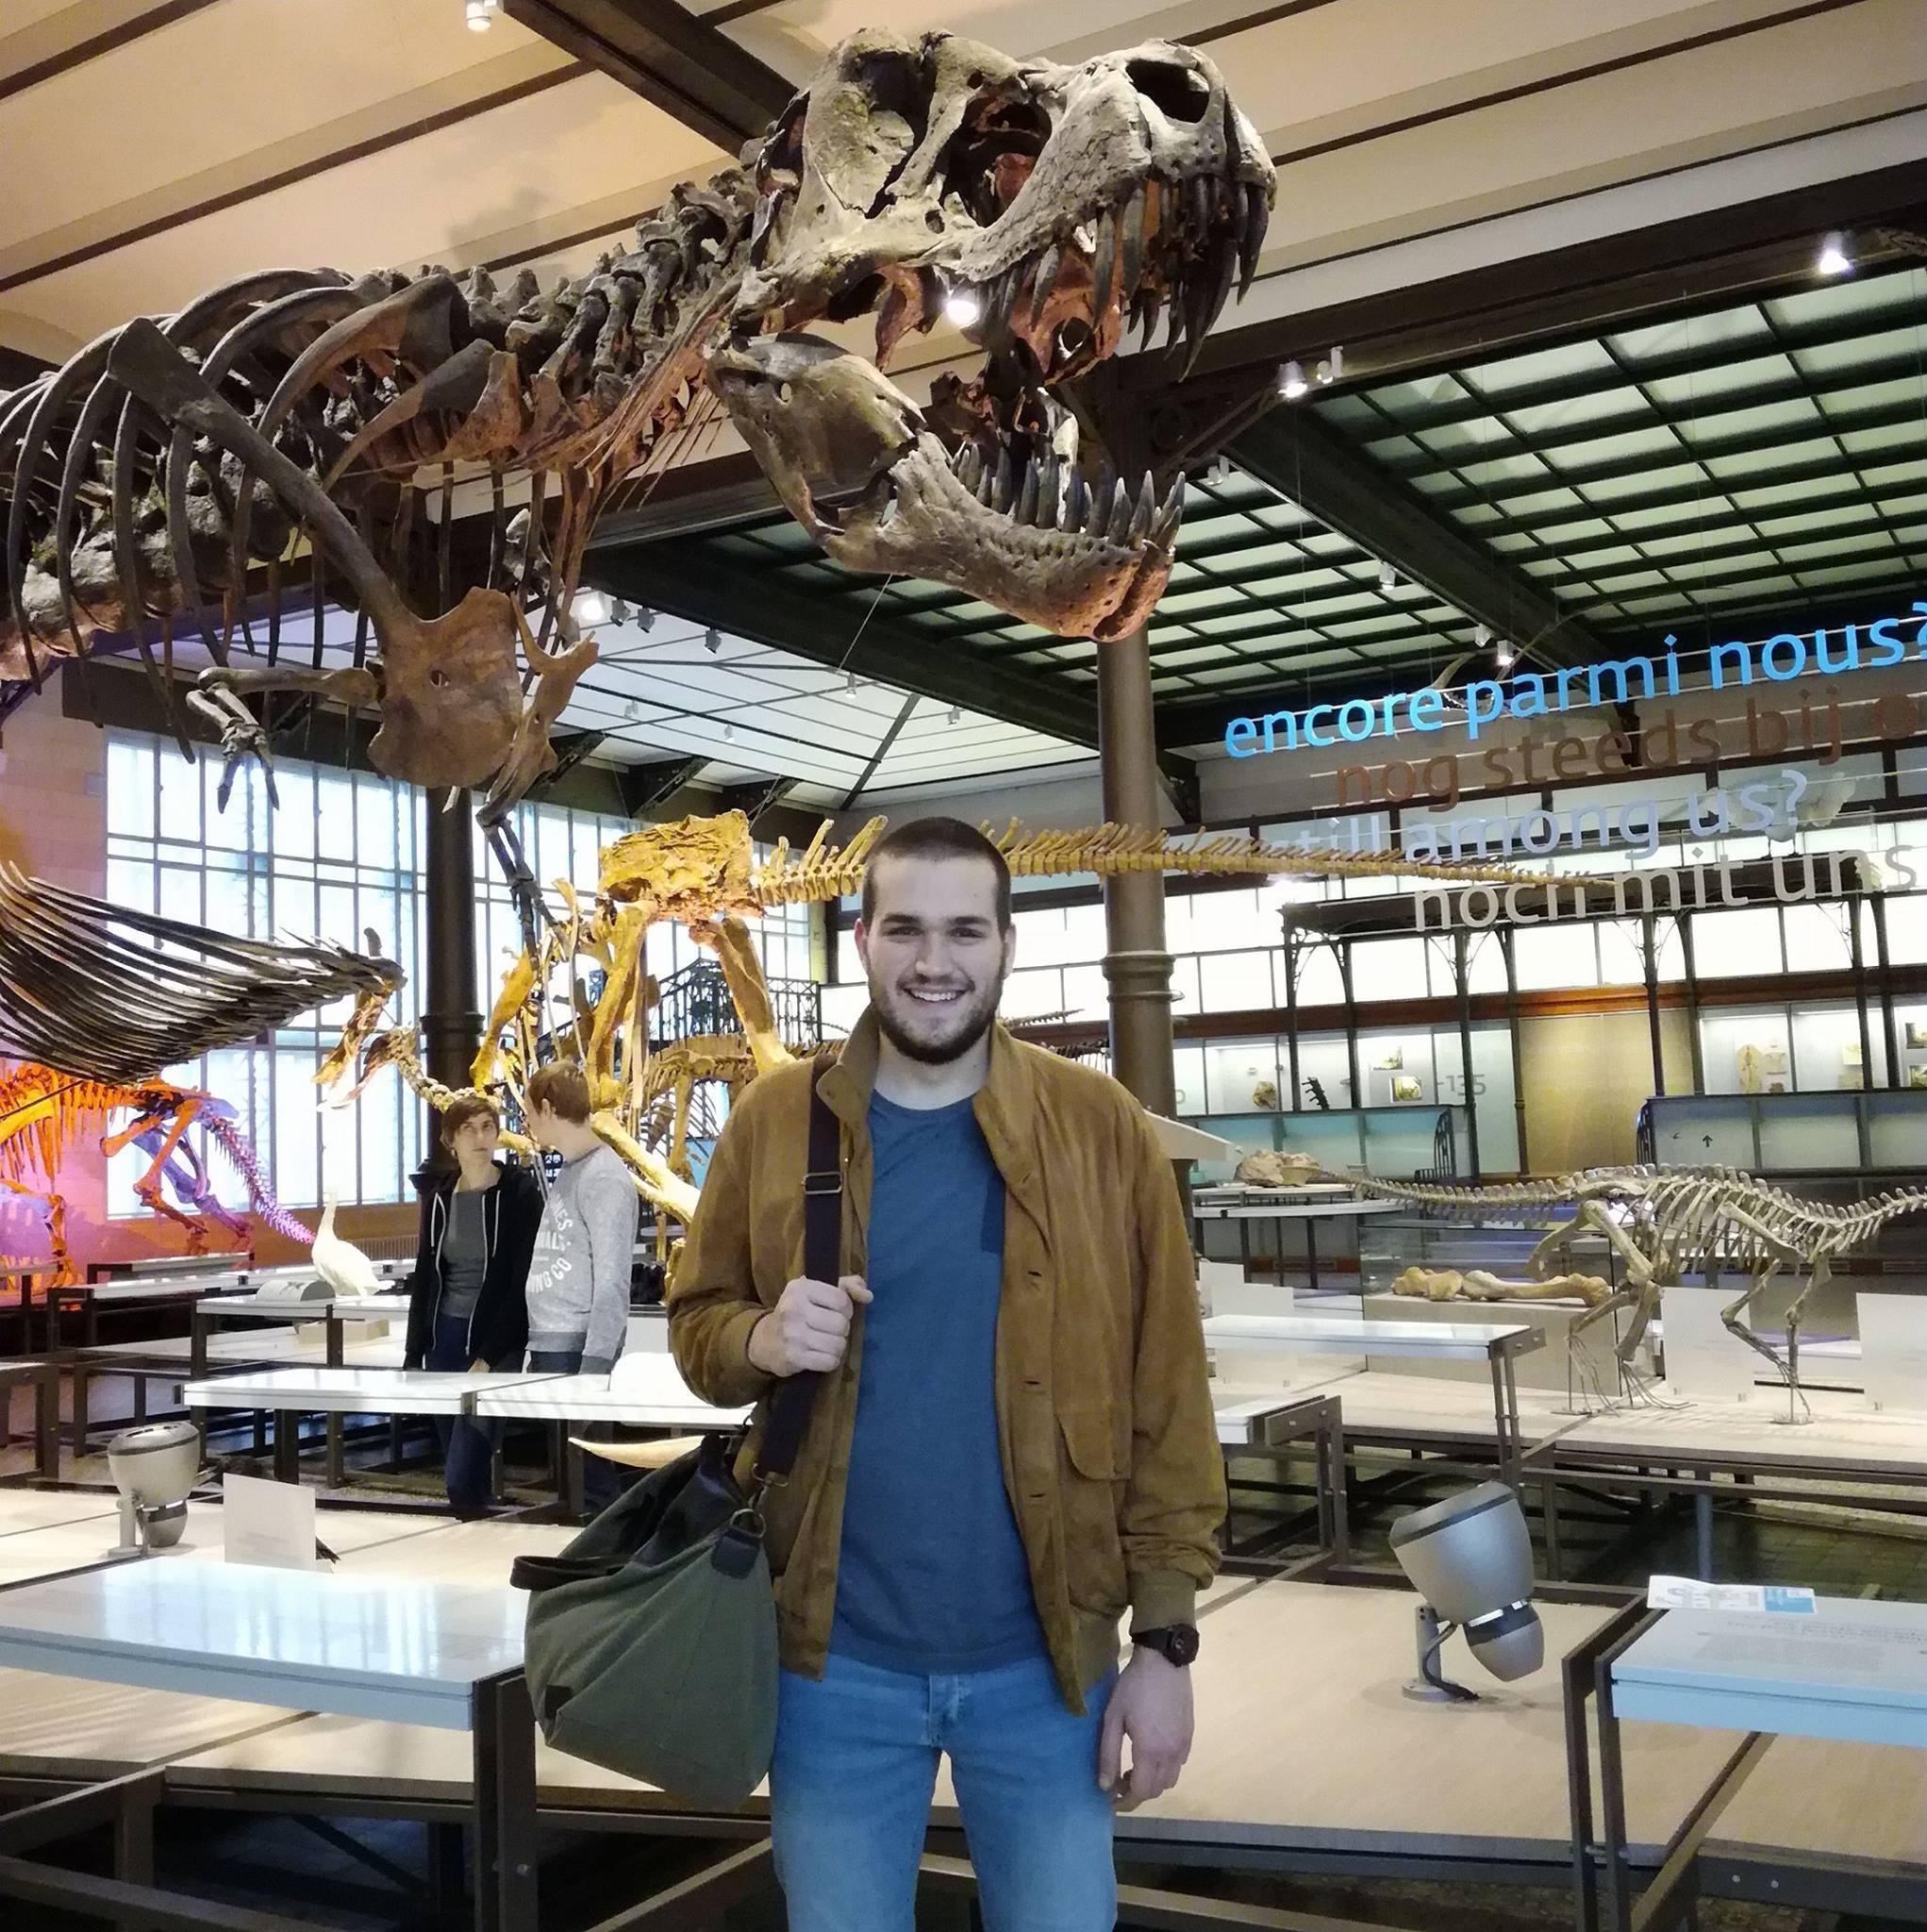
\includegraphics[width=4.00000cm]{../image/remy.jpg}

Rémy Dugauquier est en dernière année du master en biologie des
organismes et écologie. Il réalise son T.F.E. sur l'écologie des
organismes planctoniques en baie de Calvi, France.

\subsection{Madeleine Gille}\label{madeleine-gille}


\includegraphics[width=4.00000cm]{../image/madeleine.jpg}

Madeleine Gille est étudiante en dernière année du master en biologie
des organismes et écologie. Elle réalise son T.F.E. sur les effets d'un
stress salins (hyper et hyposalin) sur \emph{Seriatopora hystrix} (Dana,
1815).

\chapter{Introduction}\label{introduction}

Les coraux sont des animaux de l'embranchement des cnidaires, tout comme
les méduses. Les individus sont nommés « polypes » (Fig. 2.1). Au sein
des cnidaires, 1609 espèces de coraux durs (scléractiniaire
hermatypique) forment les récifs coralliens (Fig. 2.2). Les coraux durs
vivent en symbiose avec une microalgue unicellulaire les zooxanthelles
qui fournit l'énergie nécessaire à la formation de leur squelette
carbonate de calcium (Fig. 2.3).

\begin{figure}
\centering
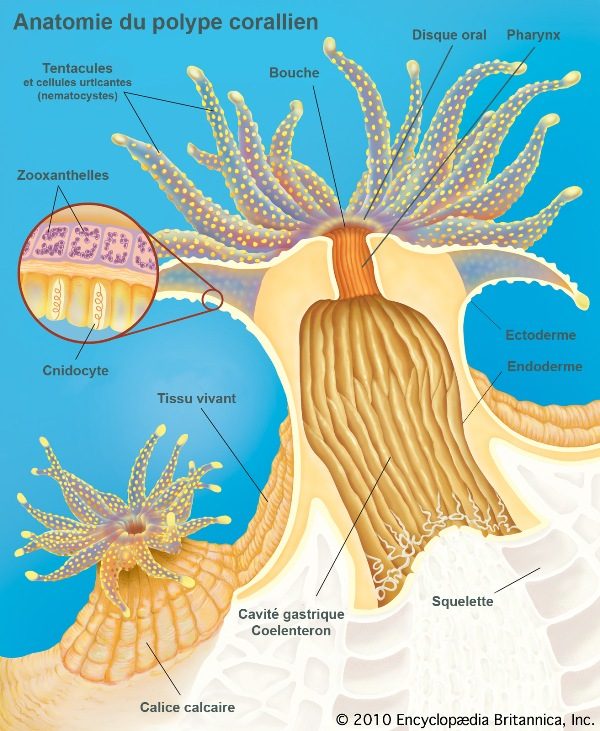
\includegraphics{../image/polype_schema.jpg}
\caption{Schéma d'un polype}
\end{figure}

\begin{figure}
\centering
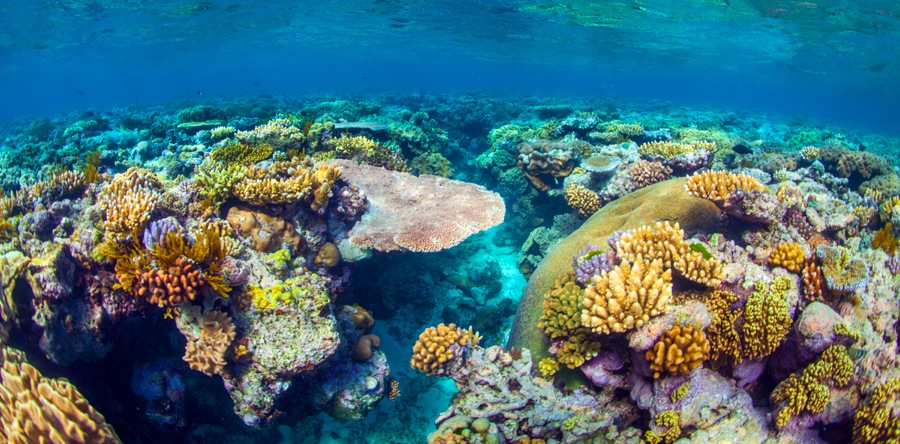
\includegraphics{../image/recif2.jpg}
\caption{Récif corallien}
\end{figure}

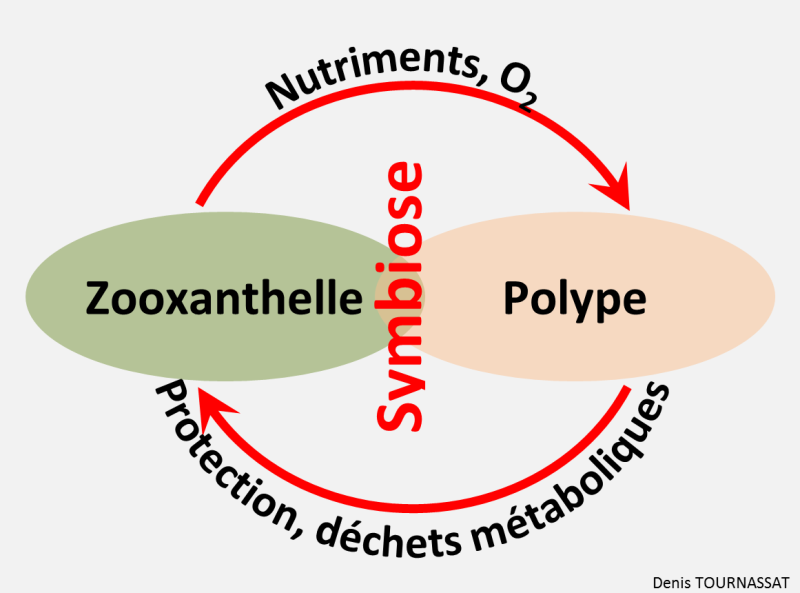
\includegraphics{../image/symbiose.png} \newpage
\null

Les récifs coralliens fournissent d'importantes niches écologiques à de
nombreux animaux qui en sont dépendants. Il est donc crucial de les
protéger.\\
En situation de stress le corail, peut expulser ses zooxanthelles, ce
qui ne laisse paraître seulement la coloration blanche de son squelette.
Ce blanchissement affaiblit considérablement le corail (Fig. 2.4).
Divers facteurs peuvent stresser le corail : l'acidité, la salinité, la
température, la pollution, etc..

\begin{figure}
\centering
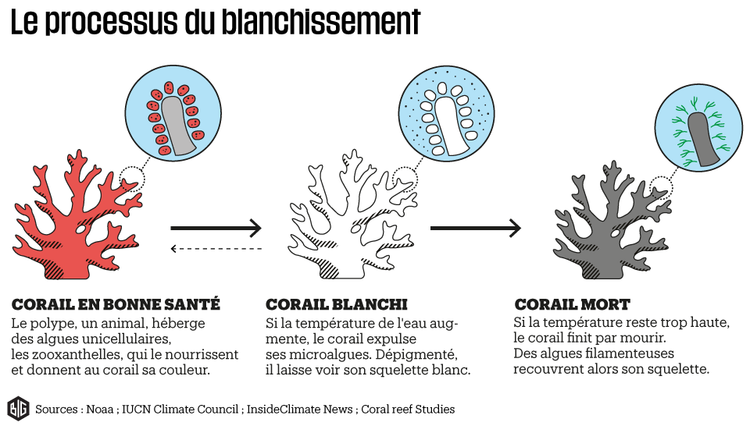
\includegraphics{../image/blanchissement.png}
\caption{Etape du blanchissement du corail}
\end{figure}

Le service d'écologie numérique des milieux aquatiques étudie en
mésocosme les réponses écophysiologiques des coraux à divers stress sur
\emph{Seriatopora hystrix} Dana 1846 principalement.

Le précédent stagiaire, Raphaël Conotte a développé une application en
local à partir du langage R permettant le monitoring des coraux (Fig.
2.5, Fig. 2.6).

Les objectifs du stage sont multiples. Premièrement, il va falloir
apprendre le langage R et ses multiples packages. Deuxièmement, se baser
sur le travail de Raphaël pour créer une version améliorée de celui-ci.
Dernièrement, une mesure régulière des coraux sera effectuée tout au
long du stage. Cela consiste à reproduire des échantillons de corails
qui seront ensuite pesé deux à trois fois par semaine, ce travail se
fait en parallèle avec la partie informatique.

L'application créée pendant ce stage aura été complètement réécrite et
simplifé. Le code de Raphaël étant beaucoup trop complexe pour un
débutant dans R.

\begin{figure}[h!]
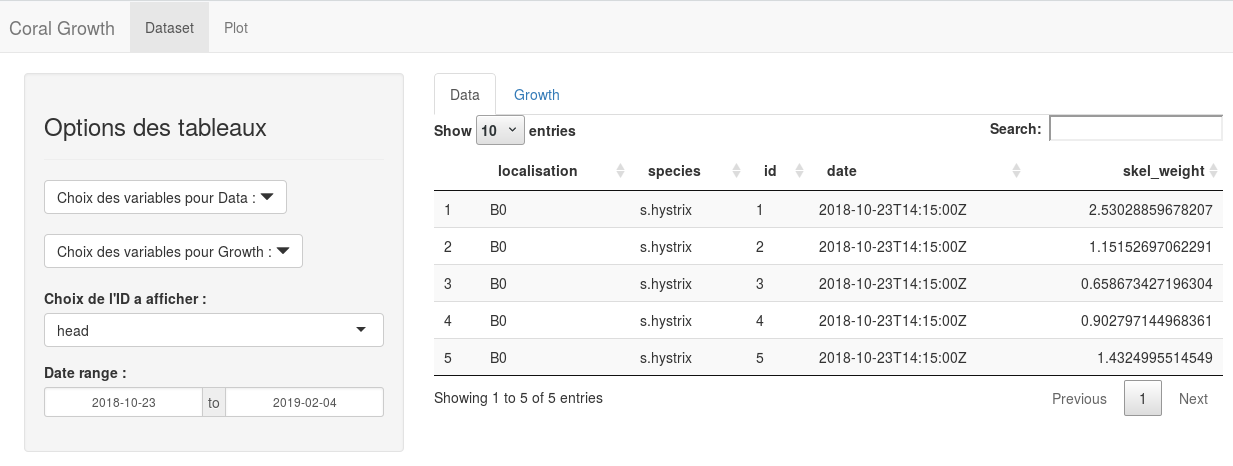
\includegraphics[]{../image/raphael1.png}
\caption{Application de Raphaël : onglet Dataset}
\end{figure}

\begin{figure}
\centering
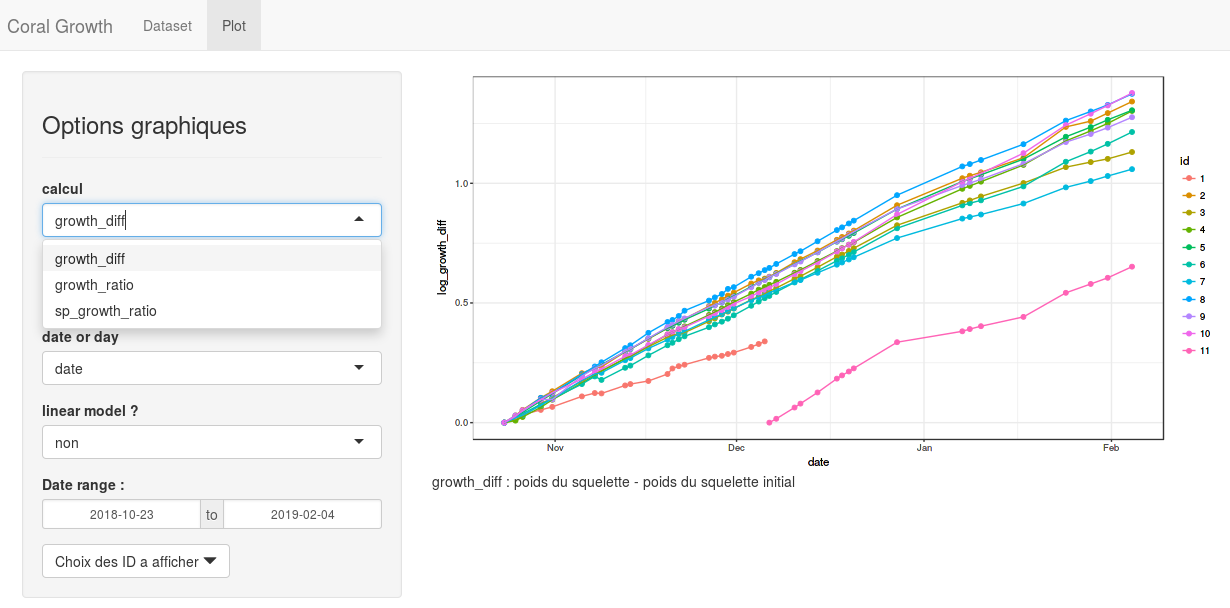
\includegraphics{../image/raphael2.png}
\caption{Application de Raphaël : onglet Plot}
\end{figure}

\chapter{Objectifs du travail}\label{objectifs-du-travail}

Le but du stage est de créer une application web via le package Shiny
dévelopé par RStudio sur R, qui suit l'évolution des coraux dans les
mésocosmes. Les coraux seront utilisés dans des expériences par le
laboratoire, il est donc nécessaire de visualiser leur croissance.
L'application doit pouvoir être utilisée facilement par d'autres
personnes à \emph{posteriori}, il faut donc l'automatiser et anticiper
les problèmes à venir.

Le stage se déroule en 2 parties, la première est une phase
d'apprentissage, la deuxième est la création de l'application et
l'implémentation d'outils pour le monitoring de la croissance des
coraux.

\section{Stage}\label{stage}

La phase d'apprentissage comprend :

\begin{itemize}
\tightlist
\item
  Apprentissage du langage de programmation R, de ses packages et de
  l'environnement RStudio.
\end{itemize}

La phase de création d'outils comprend :

\begin{itemize}
\item
  L'acquisition des données de croissance régulière des coraux.
\item
  La réalisation d'une application web Shiny, surveillant la croissance
  (monitoring) des coraux de l'espèce \emph{S. hystrix}.
\end{itemize}

\section{Outils utilisés}\label{outils-utilises}

Les outils utilisés sont :

\begin{itemize}
\item
  La machine virtuelle \emph{SciViews Box}, contenant un Linux
  (Xubuntu), R, RStudio et les paquets nécessaires pré-installés.
\item
  Les langages de programmation : R.
\item
  Les paquets : Shiny, tidyverse, ggplot2, dyplyr, plotly, googlesheets,
  ect.
\item
  Le service web GitHub.
\end{itemize}

\chapter{Résultats et
interprétations}\label{resultats-et-interpretations}

\section{Acquisition de données}\label{acquisition-de-donnees}

\subsection{Multiplication par
bouturage}\label{multiplication-par-bouturage}

Dans le but d'acquérir de nouvelles données de croissance, on a utilisé
une technique de multiplication asexuée : le bouturage. Cela consiste à
séparer à l'aide d'une pince des branches de coraux. Le nombre de
boutures s'élève à 84, toutes suspendu dans l'eau à l'aide de fil de
pêche sur une règle qui porte un numéro d'identification propre à
chacune (Fig. 4.1, Fig. 4.2).

\begin{figure}[h!]
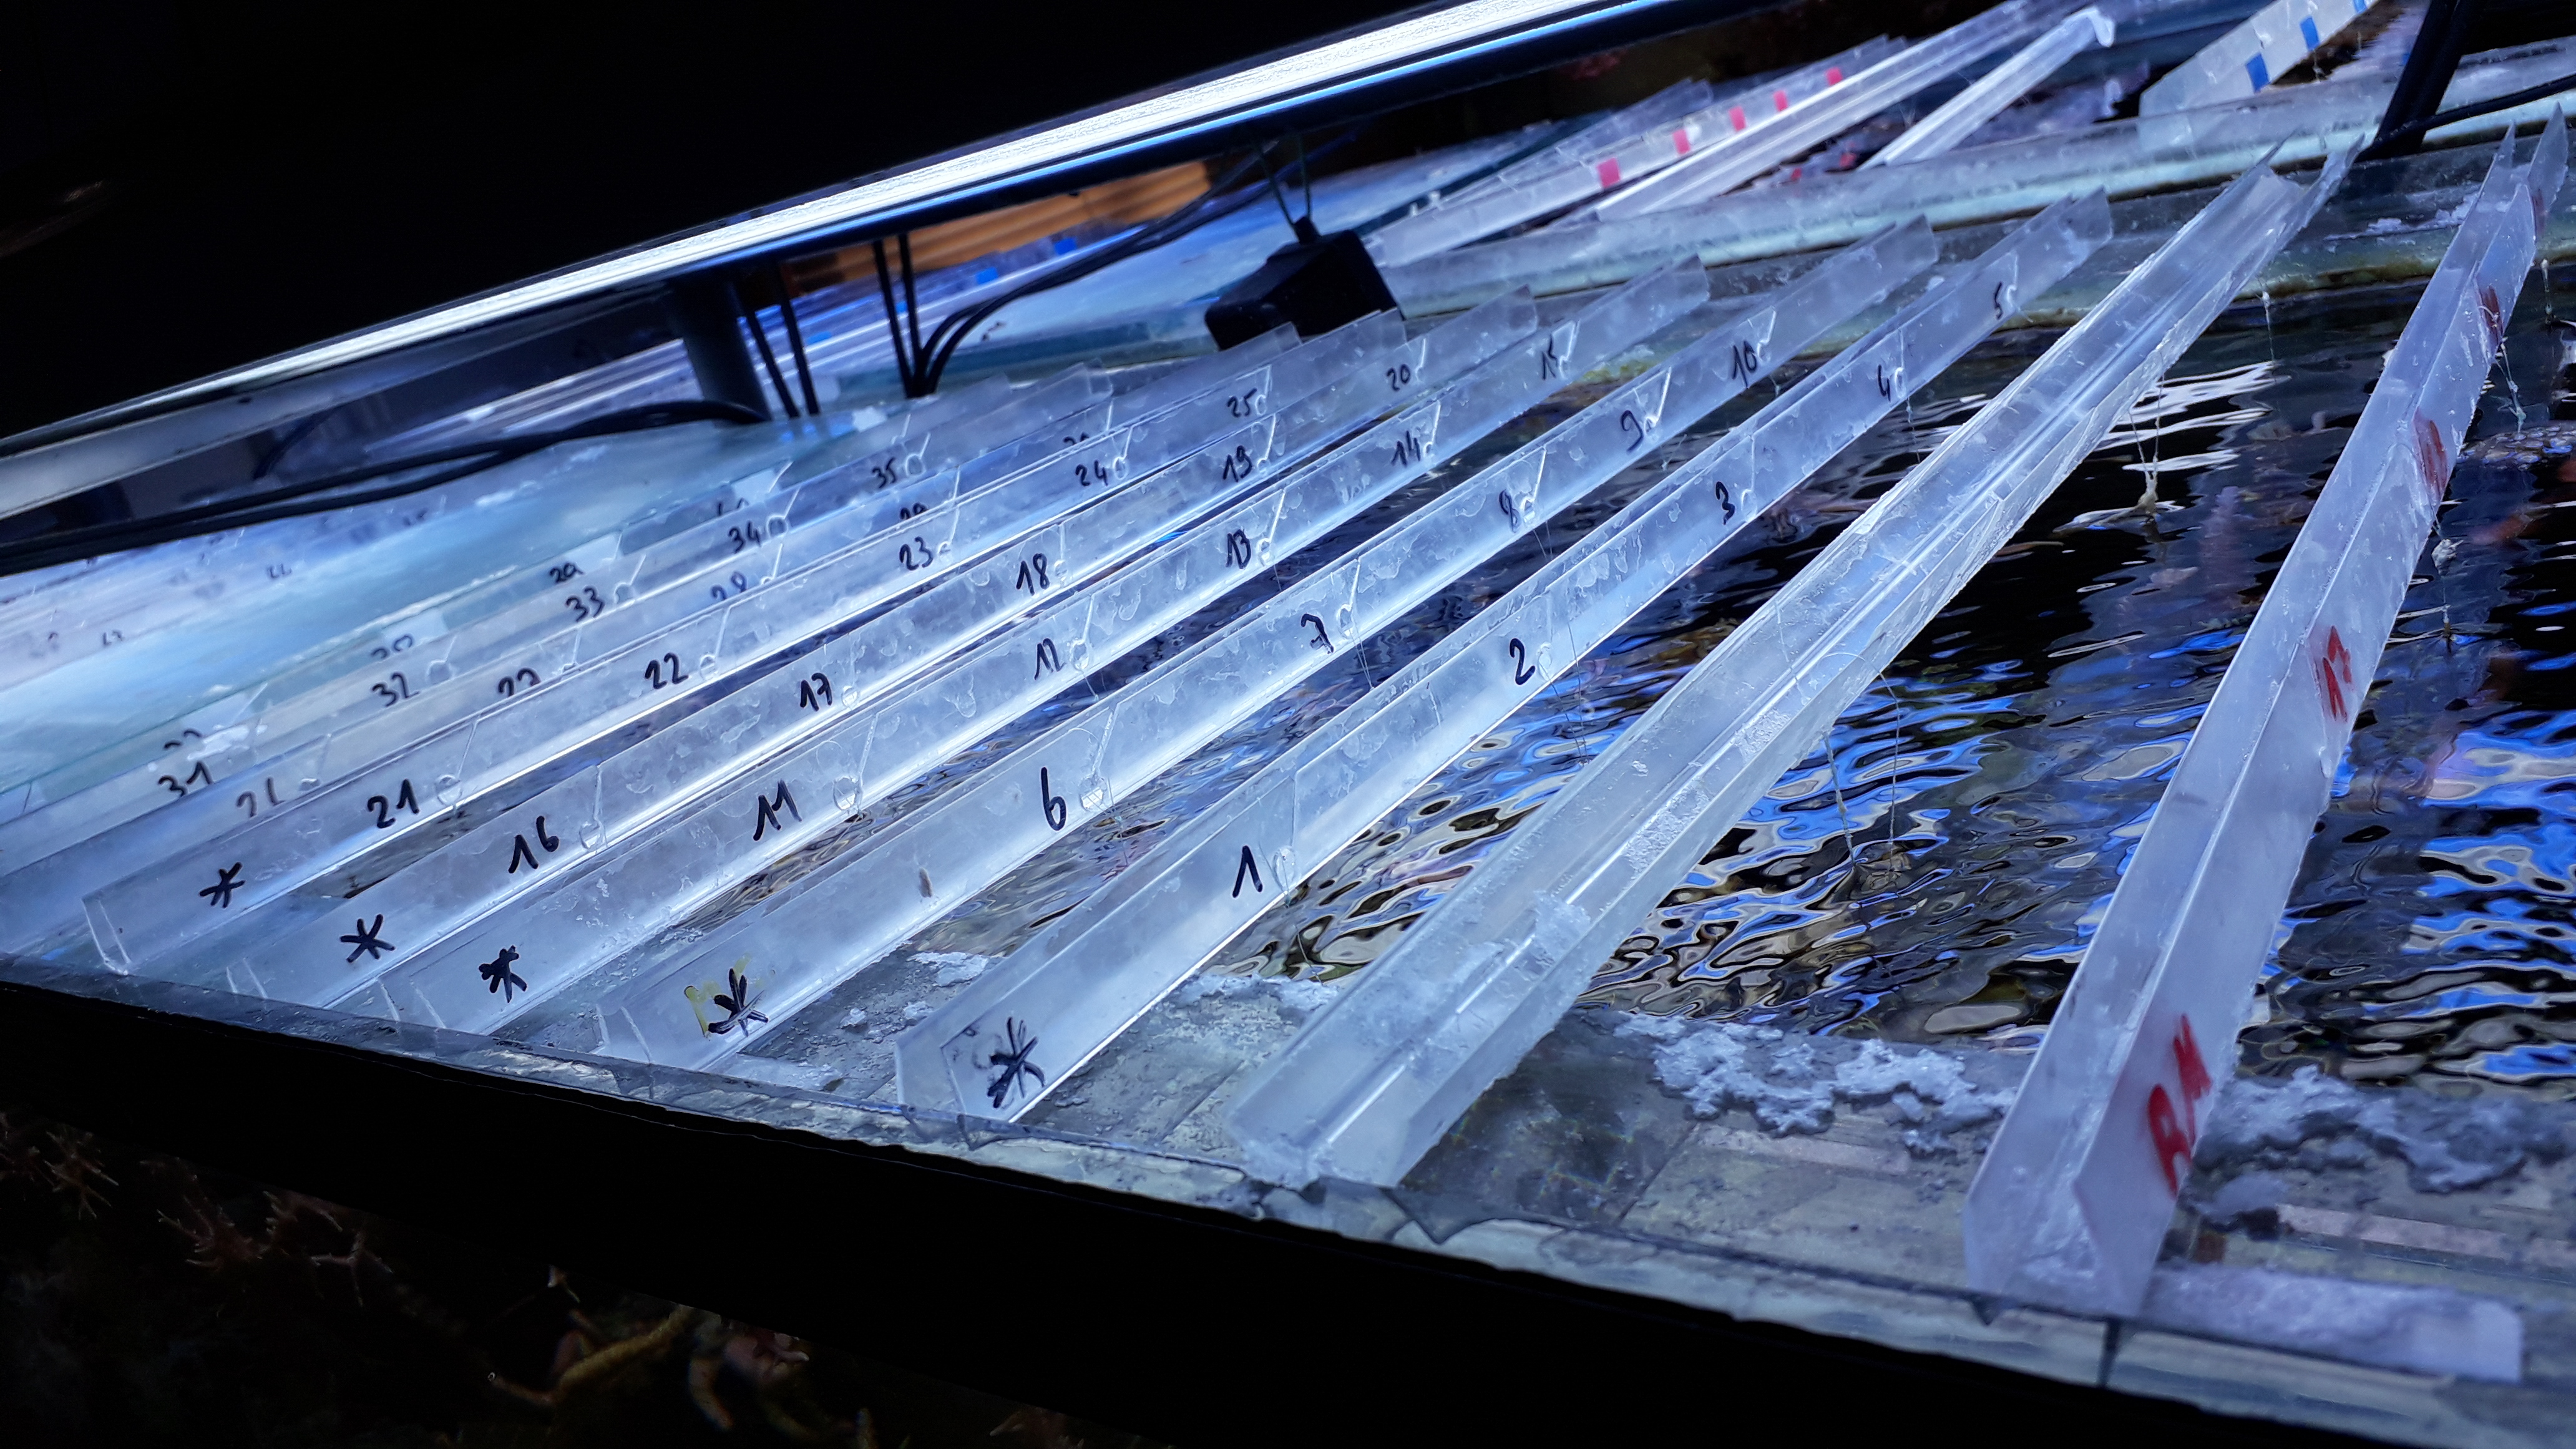
\includegraphics[]{../image/regle.jpg}
\caption{Règle numérotée}
\end{figure}

\begin{figure}[h!]
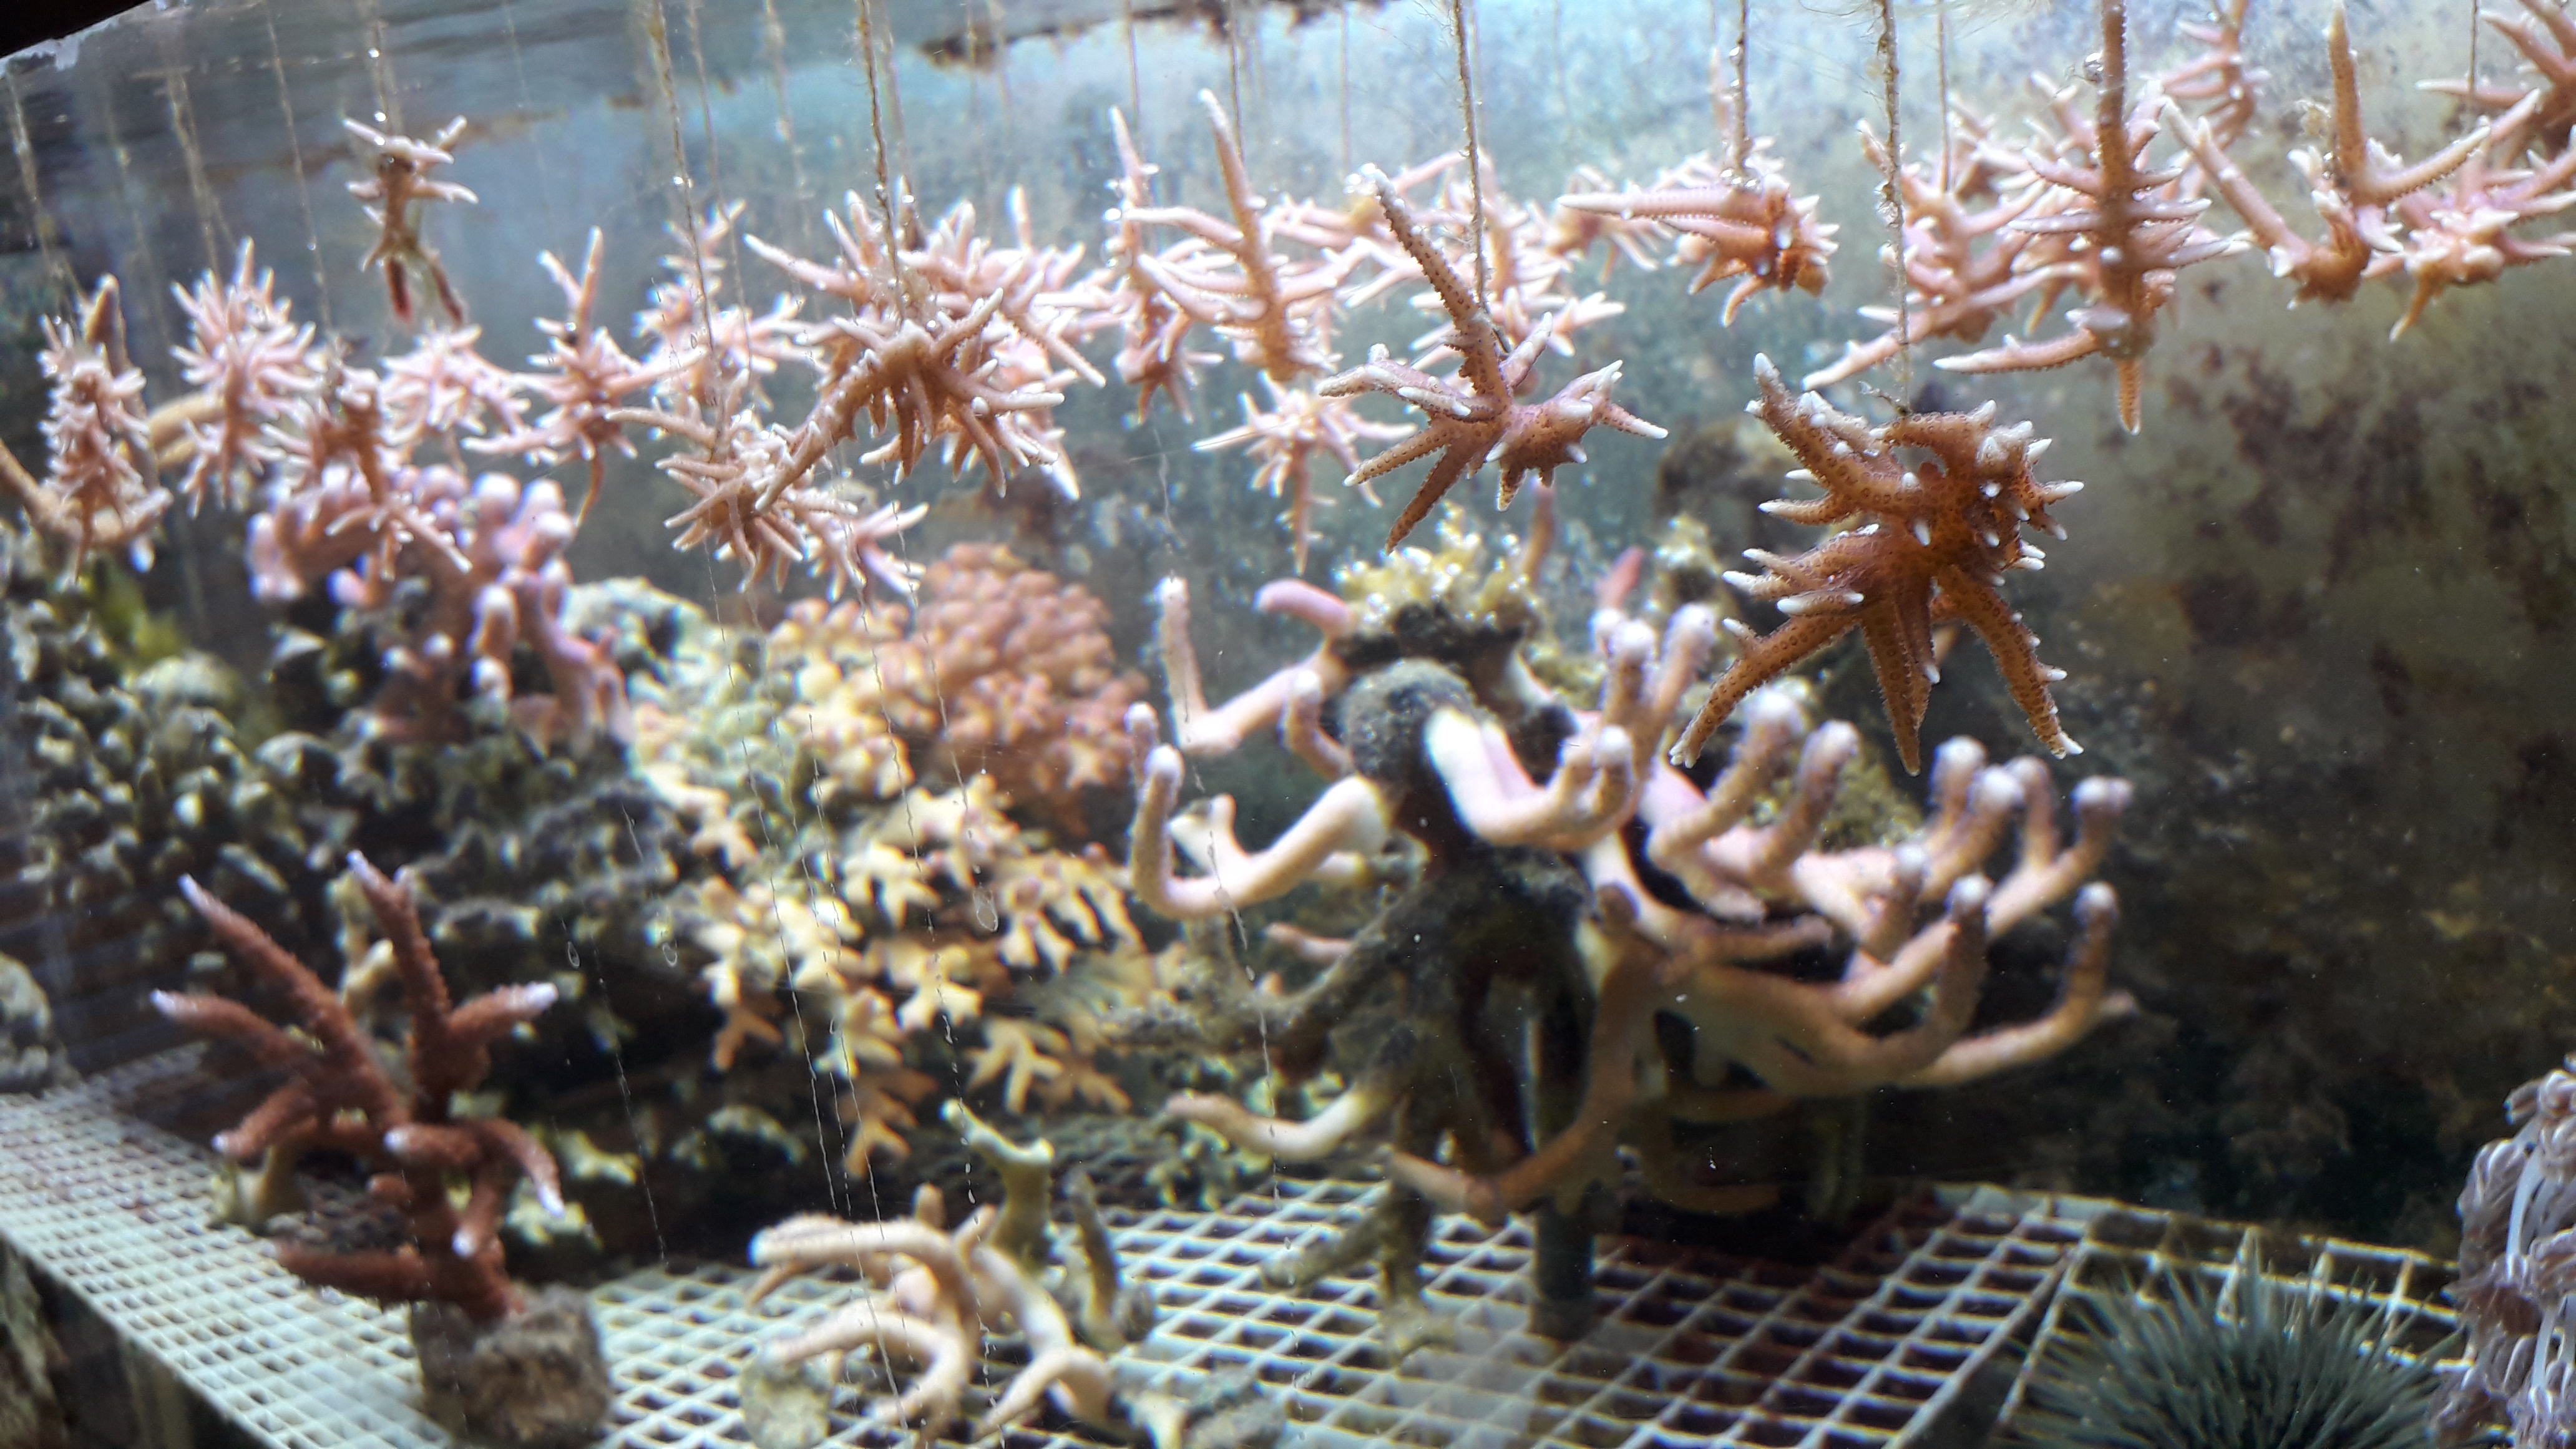
\includegraphics[]{../image/boutures.jpg}
\caption{Boutures suspendues de *Seriatopora hystrix*}
\end{figure}

\section{Outils monitorings}\label{outils-monitorings}

\subsection{Masse immergée et masse
squelettique}\label{masse-immergee-et-masse-squelettique}

Pour évaluer la croissance des boutures de coraux, on utilise la masse
squelettique. Pour l'obtenir sans détruire le corail, on mesure la masse
immergée du corail dans l'eau de mer avec une balance munie d'un crochet
(Fig. 4.3). Cette méthode de mesure est rapide et peu stressante pour
les organismes. Après avoir mesuré la température et la salinité, on
peut convertir la masse immergée en masse squelettique à l'aide de la
formule ci-dessous mise au point par Jokiel \emph{et al} (1978) :

\begin{equation}
\large
  m_{squelettique} = \frac {m_{immerge}}{ \frac{1 - \rho_{eau}}{ \rho_{squelettique}}}
\end{equation}

\(\rho_{eau}\) est déterminé par l'équation d'état de l'eau de mer grâce
à la mesure de la salinité et de la température. Le
\(\rho_{squelettique}\) est la densité de l'aragonite
(CaCO\textsubscript{3}) du squelette du corail.

\begin{figure}[h!]
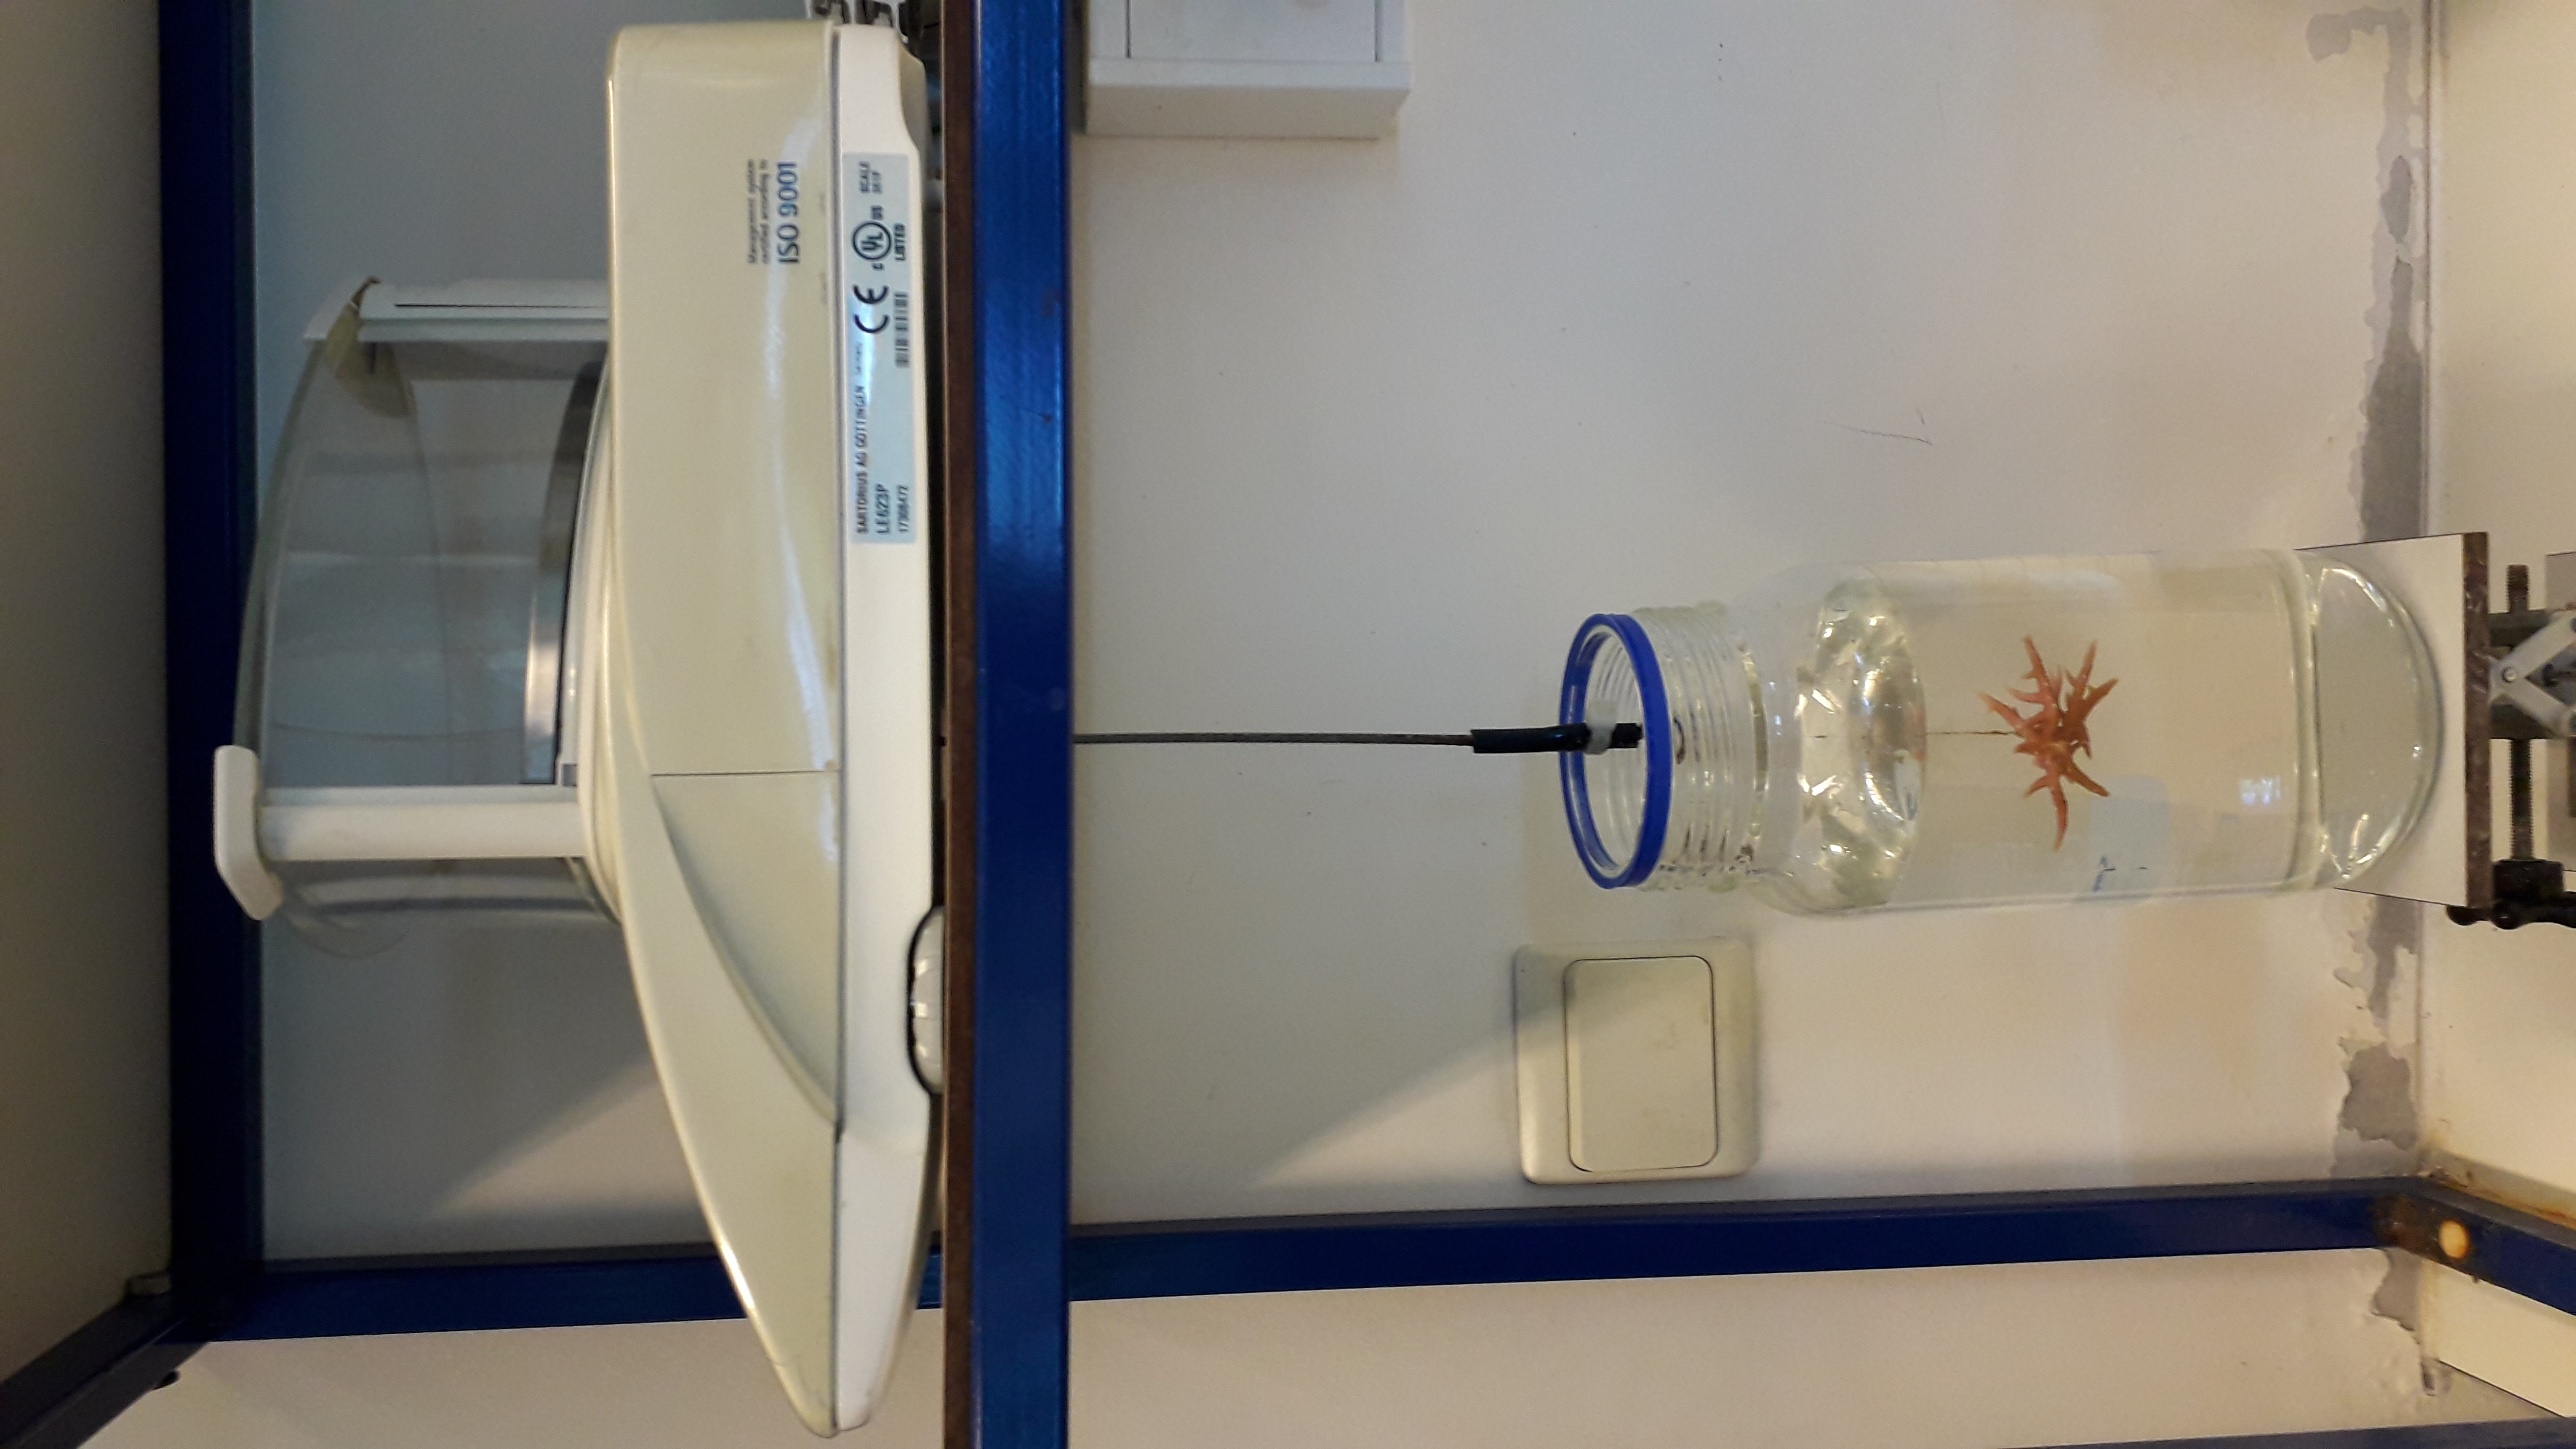
\includegraphics[]{../image/poster-balance.jpg}
\caption{Mesure du poids immergé d'une bouture}
\end{figure}

\null
\newpage

\subsection{Tableur en ligne}\label{tableur-en-ligne}

Les mesures effectuées sur les coraux et les paramètres de l'eau des
mésocosmes sont dans un premier temps notés dans un cahier de
laboratoire. Il sera nécessaire de créer un nouveau tableau de donnée
afin d'utiliser les données.

Au début, le tableur choisit était Excel, car c'est le logiciel le plus
connu et que la HEH me permet d'utiliser une licence. Cela fonctionnait
bien avec les fichiers en local. Malheureusement, aucun package permet
d'utiliser Excel en ligne.

C'est avec Googlesheets qu'une solution fut trouvé.

Le tableur est en ligne cela permet à n'importe quelle personne de
manipuler le tableau de données depuis n'importe quelle machine
connectée à internet.

Afin d'éviter au maximum des erreurs d'encodages, des règles de mise en
forme conditionnelles ont été créées pour mettre en évidence les cases
non remplies, formater le type des cellules et mettre un dégradé de
couleur suivant l'avancement des données (Fig. 4.4).

\begin{figure}[h!]
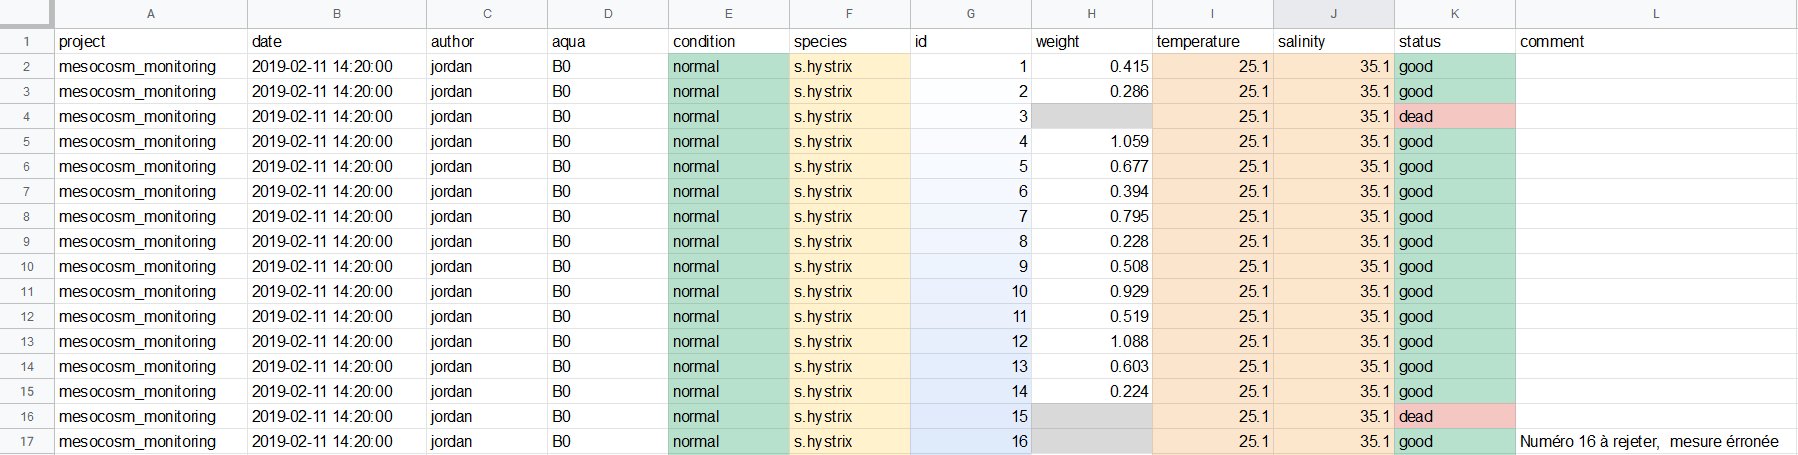
\includegraphics[width=18cm, height=15cm]{../image/tableur-gs.PNG}
\caption{Tableur en ligne Google Sheets}
\end{figure}

Le tableur est divisé en 12 colonnes :

\begin{itemize}
\tightlist
\item
  project : différencie chaque expérience réalisée, généralement on
  préfèrera recréer un nouveau tableur pour chacune des expériences
\item
  date : date et heure à laquelle les relevés de mesures ont été prises
\item
  author : nom de la personne ayant encodé dans le tableur
\item
  aqua : nom du mésocosme où la bouture a été prélevé
\item
  condition : condition spécifique appliquée à la bouture (exemple :
  stress hypersalin)
\item
  species : nom de l'espèce mesurée
\item
  id : numéro de la bouture mesurée
\item
  weight : masse immergée mesurée
\item
  temperature : température de l'eau de mer
\item
  salinity : salinité de l'eau de mer
\item
  status : état de santé de la bouture
\item
  comment : commentaire
\end{itemize}

\section{Présentation de l'application
Shiny}\label{presentation-de-lapplication-shiny}

L'application est divisée en deux fichiers, une partie ``ui'' (User
Interface), c'est la partie qui affiche les éléments graphiques de
l'interface Shiny à l'utilisateur et une partie ``server'', qui contient
toutes les commandes R qui s'opère côté serveur.

Il est possible mettre l'intégralité du code dans un seul fichier app.R.
Cependant, j'ai divisé mon script en deux fichiers ui.R et server.R pour
plus de clarté (voir partie annexe).

\vspace{1 cm}

Mon application présente 3 onglets, le premier créer un graphique
interactif (Fig. 4.5).

\begin{figure}[h!]
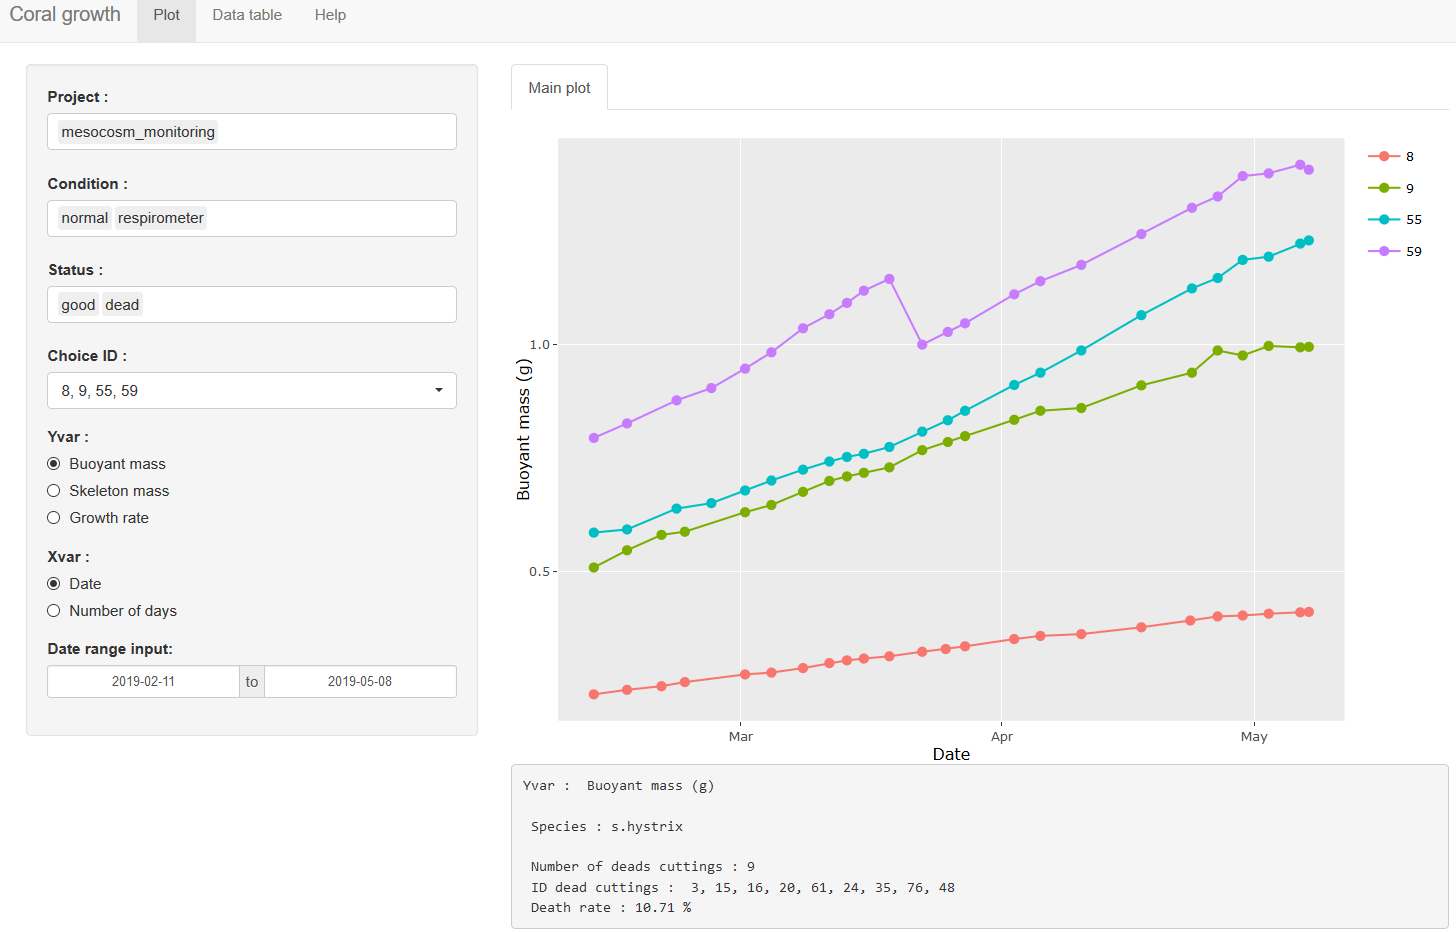
\includegraphics[]{../image/notebook-plot1.PNG}
\caption{Application Shiny : onglet "Plot"}
\end{figure}

\vspace{0.5 cm}

Par défaut, le graphique utilise en ordonnée la masse immergée des
boutures et en abscisse la date de la mesure. Les boutures sélectionnées
sont peu nombreuses pour l'exemple, mais il est possible de toutes les
sélectionner.

\vspace{0.5 cm}

Différents paramètres peuvent modifier le graphique (Fig. 4.6).

\begin{figure}
\centering
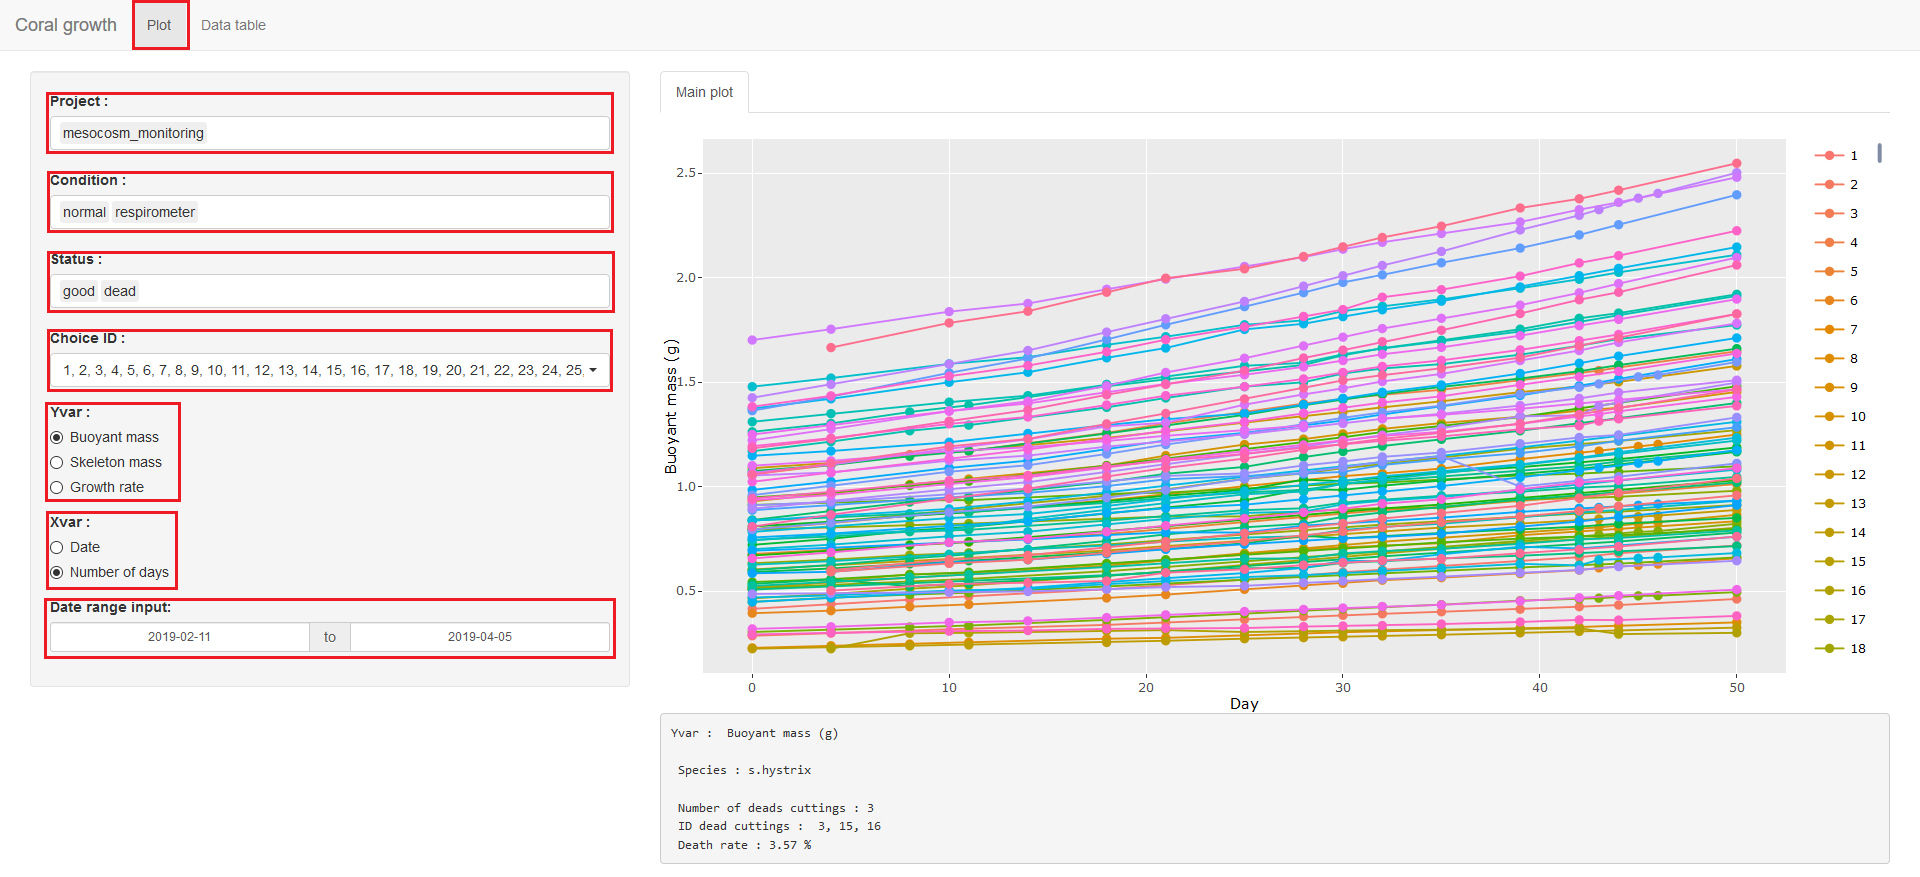
\includegraphics[width=15.00000cm]{../image/notebook-plot2.PNG}
\caption{Application Shiny : paramètres}
\end{figure}

\vspace{0.5cm}

\null
\newpage

En ordonné, on peut choisir :

\begin{itemize}
\tightlist
\item
  la masse immergée
\item
  la masse squelettique
\item
  le taux de croissance (Fig. 4.7) 
\end{itemize}

\begin{figure}[h!]
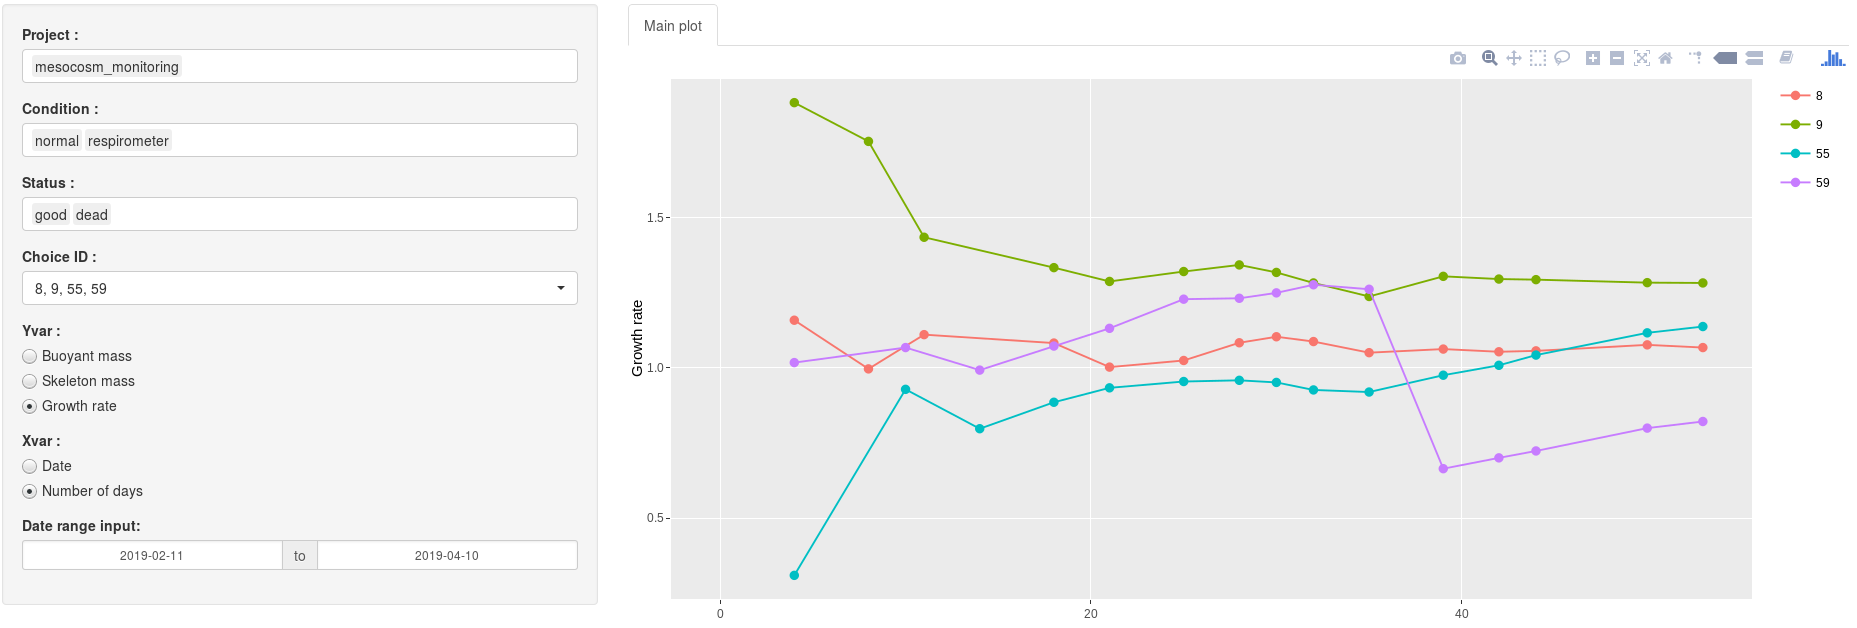
\includegraphics[]{../image/taux-croissance.PNG}
\caption{Application Shiny : taux de croissance}
\end{figure}

En abscisse, on peut choisir :

\begin{itemize}
\tightlist
\item
  la date de la mesure
\item
  le nombre de jour écoulé depuis la première mesure
\end{itemize}

Il est également possible de restreindre la période de temps (option
\emph{Date range input}).

Il est aussi possible de sélectionner les ID dans un menu déroulant, on
peut également désélectionner les lignes en cliquant sur le numéro
associer à la couleur de l'ID à droite de l'écran (Fig. 4.8, Fig. 4.9).

Le menu déroulant permet de tout sélectionner ou de tout désélectionner.

\begin{figure}[h!]
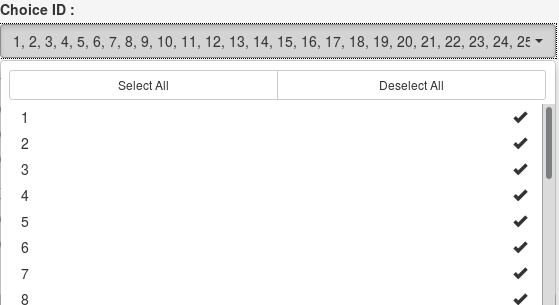
\includegraphics[]{../image/menu-deroulant.PNG}
\caption{Application Shiny : menu déroulant}
\end{figure}

En passant le curseur sur les points du graphique, on peut obtenir
quelques informations supplémentaires (Fig. 4.10).

\begin{figure}[h!]
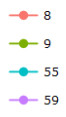
\includegraphics[]{../image/shiny-selection.PNG}
\caption{Application Shiny : affichage intéractif}
\end{figure}

\begin{figure}[h!]
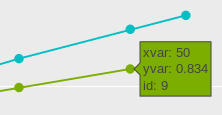
\includegraphics[]{../image/info-curseur.PNG}
\caption{Application Shiny : information via le curseur}
\end{figure}

En bas du graphique, des informations supplémentaires sont données (Fig.
4.11) :

\begin{itemize}
\tightlist
\item
  Yvar : l'ordonnée du graphique
\item
  Species : l'espèce des boutures
\item
  Number of deads cuttings : le nombre de boutures mortes
\item
  ID dead cuttings : l'ID des boutures mortes
\item
  Death rate : le taux de mortalité
\end{itemize}

\begin{figure}[h!]
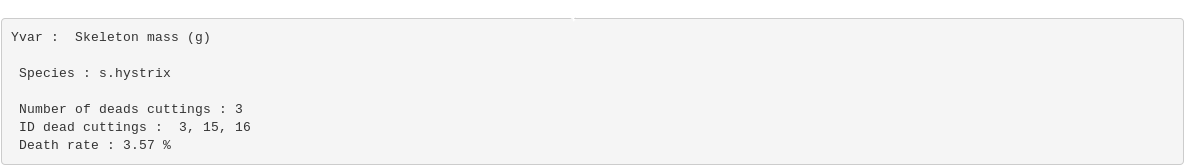
\includegraphics[]{../image/verbatim.PNG}
\caption{Application Shiny : informations supplémentaires}
\end{figure}

Le deuxième onglet contient le tableau de donnée où de nouvelles
colonnes ont été calculées, il y a l'ajout de la masse squelettique et
du ``ratio'' qui correspond au taux de croissance (Fig. 4.12).

\begin{figure}[h!]
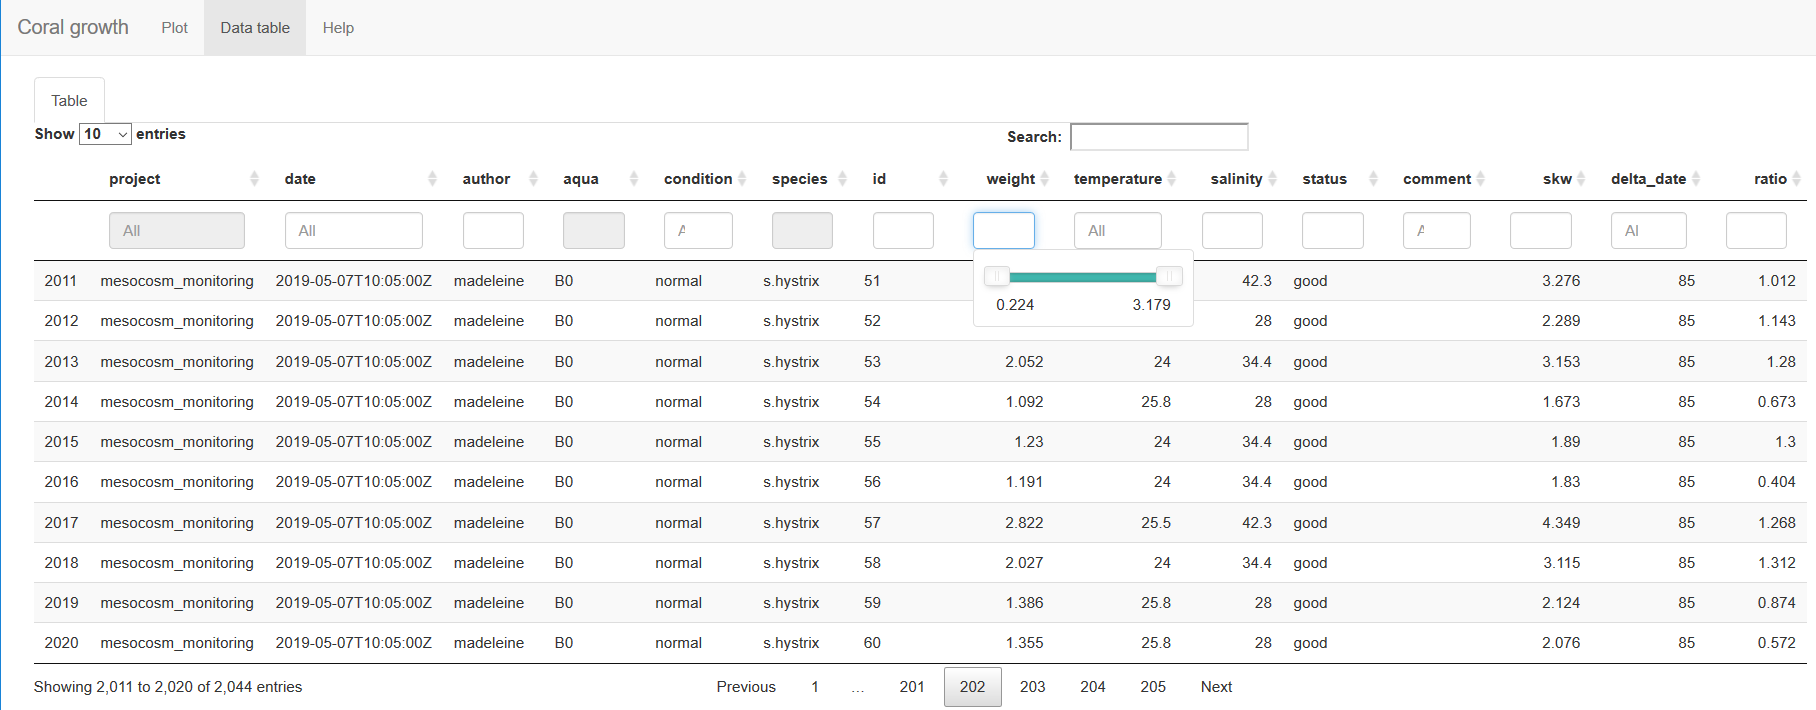
\includegraphics[]{../image/notebook-table1.png}
\caption{Application Shiny : tableau de donnée}
\end{figure}

Le dernier onglet contient une page d'aide (Fig. 4.13). Cette
documentation permettra aux utilisateurs de comprendre comment utiliser
l'application et permettra aussi de comprendre comment fonctionne le
code. Il est important de documenter son travail si l'on veut qu'il
puisse être réutilisé par la suite.

\begin{figure}[h!]
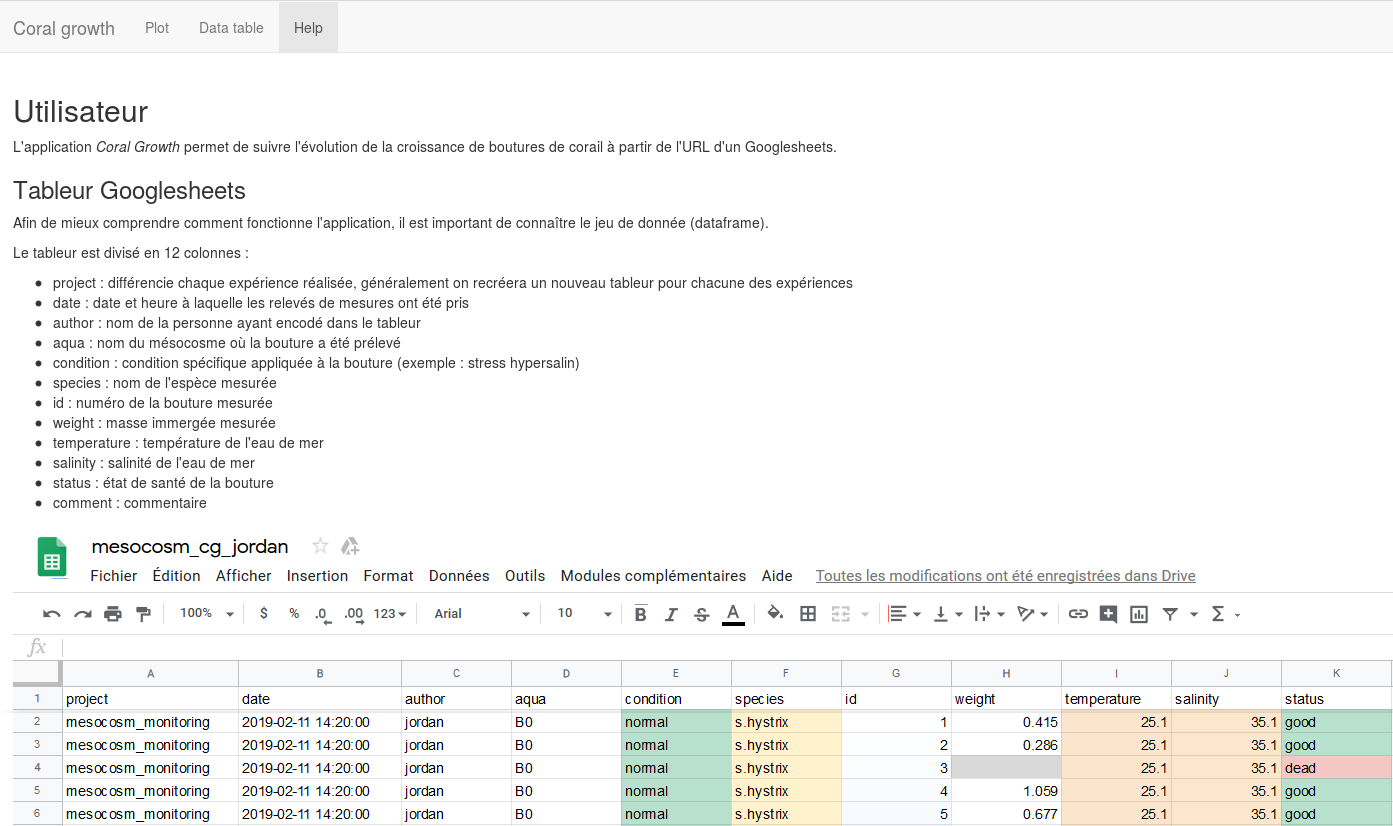
\includegraphics[]{../image/aide.PNG}
\caption{Application Shiny : onglet aide}
\end{figure}

\null
\newpage

\section{Difficultés rencontrées}\label{difficultes-rencontrees}

\subsection{R vs python}\label{r-vs-python}

La principale difficulté rencontrée au début est de passer de
l'apprentissage du langage de programmation \emph{python} à \emph{R}. Ce
sont tous les deux des langages de programmation interprétés qui peuvent
être utilisés dans le domaine du traitement de donné et de création
d'application web. \emph{python} a été créé pour faire de la
programmation informatique généraliste, il est utilisé dans de larges
domaines par des informaticiens. A l'inverse, R est dédié aux analyses
statistiques, plutôt utilisées par des spécialistes ou des
scientifiques.

Dans le domaine du \emph{data scientist}, \emph{R} et \emph{python} sont
couramment employé.

\subsection{Shiny communication entre ui.R et
server.R}\label{shiny-communication-entre-ui.r-et-server.r}

Les application web gérées par shiny utilisent deux fonctions
communiquant entre elles \textbf{ui} et le \textbf{server}.

Le schéma de communication basique entre les deux scripts commence par
la déclaration d'une variable \emph{inputId = ma\_variable} dans ui.R.
Celui-ci est appelé dans server.R sous la forme
\emph{input\$ma\_variable}, cette variable sera ensuite traitée dans un
bloc de code délimiter par des crochets.

Shiny utilise du Javascript pour dynamiser l'interface de l'utilisateur
sous une couche de code masqué, cette couche simplifie grandement le
travail avec R. Si on sort du cadre de l'utilisation prévu par Shiny, on
se heurte à de grands soucis de codage. Shiny restreint donc, la
communication entre les différents blocs de code. Dans certaines
situations cela complique le travail, ce fut notamment le cas lors de la
création du menu déroulant qui a besoin de connaître dans ui.R le nombre
d'ID qui est nécessaire, sauf que la variable donnant cette information
est dans server.R et Shiny permet difficilement de faire cela.

\section{Objectifs réalisés}\label{objectifs-realises}

Les objectifs réalisés sont :

\begin{itemize}
\item
  Bouturer les coraux et relever leurs masses immergées.
\item
  Créer un tableau de donnée en ligne contenant les données nécessaires.
\item
  Créer une application web répondant aux besoins du service à l'aide du
  paquet Shiny.
\end{itemize}

L'outil insight de Github permet de visualiser le travail des différents
contributeurs sur un même projet. On peut constater le travail réalisé
pendant le stage (Fig. 4.14).

\begin{figure}
\centering
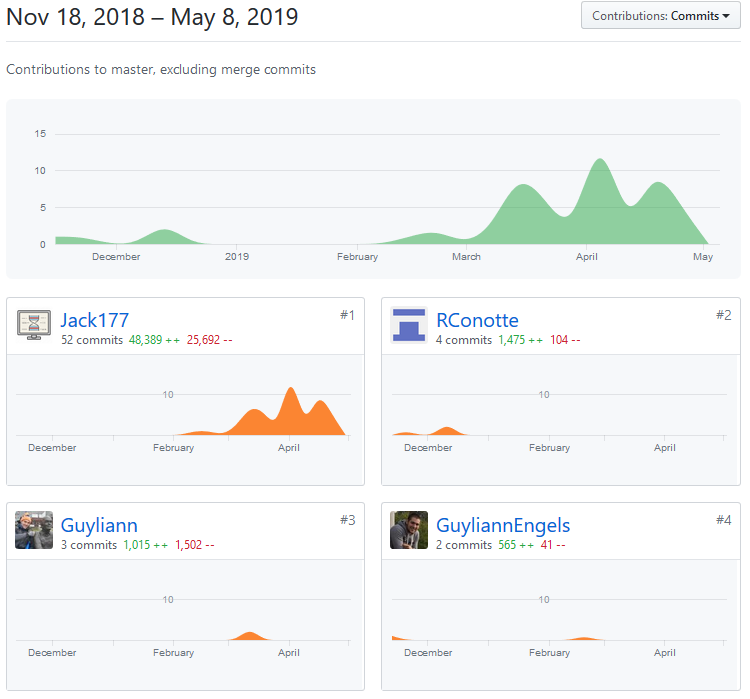
\includegraphics{../image/github.PNG}
\caption{Contributeur de l'application}
\end{figure}

\subsection{Conclusion}\label{conclusion}

L'application web répond aux attentes.

Une documentation (bookdown) est intégrée à l'application.

Elle est disponible en ligne à l'adresse :
\url{https://jack177.shinyapps.io/coralgrowth/}

Il est également possible de scanner le QR code.

\begin{figure}[h!]
\begin{centering}

\includegraphics[width=6cm]{../image/QRcode.png}
\caption{QR code}
\end{centering}
\end{figure}

\chapter{Note}\label{note}

Ce rapport en pdf intéractif a été créé en R Markdown, il permet
d'utiliser à la fois le langage LaTeX et R. LaTeX utilise des
algorithmes pour améliorer la lecture, il automatise la plupart des
paramètres comme la position des images. Il empêche parfois d'afficher
l'agencement souhaité ou il renverse des images verticales pour utiliser
au maximum l'espace de la page.

Le code en annexe a dû être retravaillé pour être correctement affiché.

La dernière version du code est disponible à l'adresse suivante :

\url{https://github.com/EcoNum/coral_growth001}

\chapter{Annexe}\label{annexe}

\section{ui.R}\label{ui.r}

\begin{Shaded}
\begin{Highlighting}[]
\KeywordTok{library}\NormalTok{(shiny)}
\KeywordTok{library}\NormalTok{(shinyWidgets)}
\KeywordTok{library}\NormalTok{(DT)}
\KeywordTok{library}\NormalTok{(plotly)}
\KeywordTok{library}\NormalTok{(shinythemes)}
\KeywordTok{library}\NormalTok{(shinyWidgets)}


\KeywordTok{shinyUI}\NormalTok{(}
  \KeywordTok{navbarPage}\NormalTok{(}
    \CommentTok{#theme = shinytheme("slate"),}
    \DataTypeTok{title =} \StringTok{"Coral growth"}\NormalTok{, }\CommentTok{# Titre onglet 1}
\NormalTok{    #### Onglet principal : Graphique}
    \KeywordTok{tabPanel}\NormalTok{(}\DataTypeTok{title =} \StringTok{"Plot"}\NormalTok{,}
\NormalTok{             ## Sidebar : volet de gauche - Input}
             \KeywordTok{sidebarPanel}\NormalTok{(}
               \KeywordTok{uiOutput}\NormalTok{(}\DataTypeTok{outputId =} \StringTok{"u_choice_project"}\NormalTok{),}
               \KeywordTok{uiOutput}\NormalTok{(}\DataTypeTok{outputId =} \StringTok{"u_choice_condition"}\NormalTok{),}
               \KeywordTok{uiOutput}\NormalTok{(}\DataTypeTok{outputId =} \StringTok{"u_choice_status"}\NormalTok{),}
               \KeywordTok{uiOutput}\NormalTok{(}\DataTypeTok{outputId =} \StringTok{"u_choice_id"}\NormalTok{), }\CommentTok{# Sélection des ID}
               \KeywordTok{uiOutput}\NormalTok{(}\DataTypeTok{outputId =} \StringTok{"u_choice_plot"}\NormalTok{)}\CommentTok{#Sélection du graphique}
               \KeywordTok{uiOutput}\NormalTok{(}\DataTypeTok{outputId =} \StringTok{"u_choice_nbr_day"}\NormalTok{),}\CommentTok{# Sélection de Xvar}
               \KeywordTok{uiOutput}\NormalTok{(}\DataTypeTok{outputId =} \StringTok{"u_choice_date"}\NormalTok{)       }\CommentTok{#Sélection date}
\NormalTok{             ),}
\NormalTok{             ## MainPanel : Volet de droite - Output}
             \KeywordTok{mainPanel}\NormalTok{(}
               \KeywordTok{tabsetPanel}\NormalTok{(}
                 \CommentTok{# Sous-onglet}
                 \KeywordTok{tabPanel}\NormalTok{(}\DataTypeTok{title =} \StringTok{"Main plot"}\NormalTok{,}
                          \KeywordTok{plotlyOutput}\NormalTok{(}\DataTypeTok{outputId =} \StringTok{"u_plot"}\NormalTok{, }
                                       \DataTypeTok{height =} \StringTok{"600px"}\NormalTok{ ),}
                          \CommentTok{#sortie console}
                          \KeywordTok{verbatimTextOutput}\NormalTok{(}\DataTypeTok{outputId =} \StringTok{"u_info"}\NormalTok{))}
                 \CommentTok{#tabPanel(title = "Test plot")}
\NormalTok{               )}
\NormalTok{             )}
\NormalTok{    ),}
\NormalTok{    ### Onglet principal : Tableau de donnée}
    \KeywordTok{tabPanel}\NormalTok{(}\StringTok{"Data table"}\NormalTok{,}
             \CommentTok{# Sidebar : Volet de gauche - Input}
             \CommentTok{# sidebarPanel(}
             \CommentTok{# ),}
             \CommentTok{# MainPanel : Volet de droite - Output}
             \KeywordTok{mainPanel}\NormalTok{(}
               \KeywordTok{tabsetPanel}\NormalTok{(}
                 \KeywordTok{tabPanel}\NormalTok{(}\DataTypeTok{title =} \StringTok{"Table"}\NormalTok{, }\KeywordTok{DTOutput}\NormalTok{(}\DataTypeTok{outputId =} \StringTok{"u_table"}\NormalTok{)}
\NormalTok{                          )}
\NormalTok{               )}
\NormalTok{             )}
\NormalTok{    ),}
    
\NormalTok{    ### Onglet principal : Aide}
    \KeywordTok{tabPanel}\NormalTok{(}\DataTypeTok{title =} \StringTok{"Help"}\NormalTok{,}
             \KeywordTok{fluidRow}\NormalTok{(}
\OperatorTok{<}\ErrorTok{<<<<<<}\StringTok{ }\NormalTok{HEAD}
               \KeywordTok{column}\NormalTok{(}\DecValTok{12}\NormalTok{, }\KeywordTok{includeMarkdown}\NormalTok{(}
                 \StringTok{"../../analysis/Notebook/Notebook-Manuel.Rmd"}\NormalTok{))))}
\OperatorTok{==}\ErrorTok{=====}
\StringTok{               }\KeywordTok{uiOutput}\NormalTok{(}\DataTypeTok{outputId =} \StringTok{"u_lien"}\NormalTok{)}
\NormalTok{             ))}
\OperatorTok{>}\ErrorTok{>>>>>>}\StringTok{ }\NormalTok{9c027f3a6d120b3a6a1d70f266e15f6a12e4e577}
  \ErrorTok{)}
\ErrorTok{)}
\end{Highlighting}
\end{Shaded}

\section{server.R}\label{server.r}

\begin{Shaded}
\begin{Highlighting}[]
\KeywordTok{library}\NormalTok{(shiny)}
\KeywordTok{library}\NormalTok{(ggplot2)}
\KeywordTok{library}\NormalTok{(lubridate)}
\KeywordTok{library}\NormalTok{(tidyverse)}
\KeywordTok{library}\NormalTok{(dplyr)}
\KeywordTok{library}\NormalTok{(plotly)}
\KeywordTok{library}\NormalTok{(shinyWidgets)}
\NormalTok{SciViews}\OperatorTok{::}\NormalTok{R}



\NormalTok{### ------------------__Partie logique du serveur__-----------------------}
\KeywordTok{shinyServer}\NormalTok{(}\ControlFlowTok{function}\NormalTok{(input, output, session) \{}

  \CommentTok{# Tableur de Madeleine :}
  \CommentTok{# coral_url <- "https://docs.google.com/spreadsheets/d/e/2PACX-1vTJLtfjj}
  \CommentTok{#UM4VK6aM177ly9GCKyMHFrFqQdsqjhJCtpe4DUGuZWOe2fZWB5xTZEx3WAcW08BVEBFfn2C}
  \CommentTok{#/pub?gid=0&single=true&output=csv"}

  \CommentTok{# Tableur de Jordan :}
\NormalTok{  coral_url <-}\StringTok{ "https://docs.google.com/spreadsheets/d/e/2PACX-1vSoBfvhztF}
\StringTok{  gALk1fcljBbYP03D-fRIEy7mu1DrHKZ--BXYZWHFxUujac_-gFSteM99p7CFQILT_eXcC/pu}
\StringTok{  b?gid=0&single=true&output=csv"}

  \CommentTok{#Importation et format des colonnes}
  \KeywordTok{read_csv}\NormalTok{(coral_url,}
           \DataTypeTok{col_types =} \KeywordTok{cols}\NormalTok{( }\DataTypeTok{.default =} \KeywordTok{col_character}\NormalTok{(),}
                             \DataTypeTok{date =} \KeywordTok{col_datetime}\NormalTok{(),}
                             \DataTypeTok{weight =} \KeywordTok{col_double}\NormalTok{(),}
                             \DataTypeTok{temperature =} \KeywordTok{col_double}\NormalTok{(),}
                             \DataTypeTok{salinity =} \KeywordTok{col_double}\NormalTok{() )) }\OperatorTok
\StringTok{    }\KeywordTok{mutate}\NormalTok{(.,}
           \DataTypeTok{project =} \KeywordTok{factor}\NormalTok{(project), }\DataTypeTok{author =} \KeywordTok{factor}\NormalTok{(author),}
           \DataTypeTok{aqua =} \KeywordTok{factor}\NormalTok{(aqua),}
           \DataTypeTok{condition =} \KeywordTok{factor}\NormalTok{(condition),}
           \DataTypeTok{species =} \KeywordTok{factor}\NormalTok{(species),}
           \DataTypeTok{id =} \KeywordTok{factor}\NormalTok{(id, }\DataTypeTok{levels =} \DecValTok{1}\OperatorTok{:}\KeywordTok{length}\NormalTok{(}\KeywordTok{unique}\NormalTok{(id))),}
           \DataTypeTok{status =} \KeywordTok{factor}\NormalTok{(status)}
\NormalTok{    ) ->}\StringTok{ }\NormalTok{df}

\NormalTok{  ### Calcul du poids squelettique :}
  \CommentTok{#a corriger : rho_aragonite}
  \CommentTok{#P = Pression hydrostatique, elle vaut 0 a la surface}
\NormalTok{  skeleton_weight <-}\StringTok{ }\ControlFlowTok{function}\NormalTok{(S, T, }\DataTypeTok{P =} \DecValTok{0}\NormalTok{,}
\NormalTok{                              buoyant_weight,}
                              \DataTypeTok{rho_aragonite =} \DecValTok{2930}\NormalTok{)\{}
\NormalTok{    rho_water <-}\StringTok{ }\NormalTok{seacarb}\OperatorTok{::}\KeywordTok{rho}\NormalTok{(}\DataTypeTok{S =}\NormalTok{ S, }\DataTypeTok{T =}\NormalTok{ T , }\DataTypeTok{P =}\NormalTok{ P)}
\NormalTok{    skl_wgt <-}\StringTok{ }\NormalTok{buoyant_weight }\OperatorTok{/}\StringTok{ }\NormalTok{(}\DecValTok{1} \OperatorTok{-}\StringTok{ }\NormalTok{(rho_water }\OperatorTok{/}\StringTok{ }\NormalTok{rho_aragonite))}
\NormalTok{    skl_wgt <-}\StringTok{ }\KeywordTok{round}\NormalTok{(skl_wgt, }\DataTypeTok{digits =} \DecValTok{3}\NormalTok{)}
    \KeywordTok{return}\NormalTok{(skl_wgt)}
\NormalTok{  \}}

  \CommentTok{# Ajout de la colonne du poids squelettique}
\NormalTok{  df <-}\StringTok{ }\KeywordTok{mutate}\NormalTok{(df,}
                  \DataTypeTok{skw =} \KeywordTok{skeleton_weight}\NormalTok{(}\DataTypeTok{S =}\NormalTok{ salinity,}
                                        \DataTypeTok{T =}\NormalTok{ temperature,}
                                        \DataTypeTok{buoyant_weight =}\NormalTok{ weight))}

  \CommentTok{# Nombre de ID different}
\NormalTok{  nbr_id <-}\StringTok{ }\KeywordTok{unique}\NormalTok{(df}\OperatorTok{$}\NormalTok{id)}

  \CommentTok{# Conditions}
\NormalTok{  nbr_condition <-}\StringTok{ }\KeywordTok{unique}\NormalTok{(df}\OperatorTok{$}\NormalTok{condition)}

  \CommentTok{# Projet}
\NormalTok{  nbr_projet <-}\StringTok{ }\KeywordTok{unique}\NormalTok{(df}\OperatorTok{$}\NormalTok{project)}

  \CommentTok{# Statut}
\NormalTok{  nbr_status <-}\StringTok{ }\KeywordTok{unique}\NormalTok{(df}\OperatorTok{$}\NormalTok{status)}

  \CommentTok{# Taux de croissance}
\NormalTok{  df }\OperatorTok
\StringTok{    }\KeywordTok{group_by}\NormalTok{(., id) }\OperatorTok
\StringTok{    }\KeywordTok{arrange}\NormalTok{(., date) }\OperatorTok
\StringTok{    }\KeywordTok{mutate}\NormalTok{(.,}
           \DataTypeTok{delta_date =}\NormalTok{ (}\KeywordTok{as.numeric}\NormalTok{(}\KeywordTok{difftime}\NormalTok{(date, }
\NormalTok{                                             date[}\DecValTok{1}\NormalTok{], }\DataTypeTok{units =} \StringTok{"days"}\NormalTok{))),}
           \DataTypeTok{ratio =} \KeywordTok{round}\NormalTok{(((skw}\OperatorTok{-}\NormalTok{skw[}\DecValTok{1}\NormalTok{])}\OperatorTok{/}\NormalTok{skw[}\DecValTok{1}\NormalTok{]}\OperatorTok{/}\NormalTok{delta_date)}\OperatorTok{*}\DecValTok{100}\NormalTok{,}\DataTypeTok{digits =} \DecValTok{3}\NormalTok{),}
           \DataTypeTok{delta_date =} \KeywordTok{round}\NormalTok{(delta_date, }\DataTypeTok{digits =} \DecValTok{0}\NormalTok{)) }\OperatorTok
\StringTok{    }\KeywordTok{ungroup}\NormalTok{(.) ->}\StringTok{ }\NormalTok{df}


\NormalTok{  ### ----------__Fin traitement du tableau de données__ ------------- }\AlertTok{###}

  \CommentTok{#======================================================================#}

  \CommentTok{# ----------------------- Selection des dates --------------------------}
\NormalTok{  output}\OperatorTok{$}\NormalTok{u_choice_date <-}\StringTok{ }\KeywordTok{renderUI}\NormalTok{(\{}

    \KeywordTok{dateRangeInput}\NormalTok{(}\DataTypeTok{inputId =} \StringTok{"s_choice_date"}\NormalTok{,}
                   \DataTypeTok{label =} \StringTok{'Date range input: '}\NormalTok{,}
                   \DataTypeTok{start =} \KeywordTok{min}\NormalTok{(df}\OperatorTok{$}\NormalTok{date), }\DataTypeTok{end =} \KeywordTok{max}\NormalTok{(df}\OperatorTok{$}\NormalTok{date),}
                   \DataTypeTok{min =} \KeywordTok{min}\NormalTok{(df}\OperatorTok{$}\NormalTok{date), }\DataTypeTok{max =} \KeywordTok{Sys.Date}\NormalTok{()}
\NormalTok{    )}
\NormalTok{  \})}
  \CommentTok{# ------------------------- Selection Xvar -----------------------------}
\NormalTok{  output}\OperatorTok{$}\NormalTok{u_choice_nbr_day <-}\StringTok{ }\KeywordTok{renderUI}\NormalTok{(\{}

    \KeywordTok{radioButtons}\NormalTok{(}\DataTypeTok{inputId =} \StringTok{"s_choice_nbr_day"}\NormalTok{,}
                 \DataTypeTok{label =} \StringTok{'Xvar : '}\NormalTok{,}
                 \DataTypeTok{choices =} \KeywordTok{c}\NormalTok{(}\StringTok{"Date"}\NormalTok{, }\StringTok{"Number of days"}\NormalTok{),}
                 \DataTypeTok{selected =} \StringTok{"Number of days"}
\NormalTok{    )}
\NormalTok{  \})}

  \CommentTok{#--------------------------Selection id---------------------------------}
\NormalTok{  output}\OperatorTok{$}\NormalTok{u_choice_id <-}\StringTok{ }\KeywordTok{renderUI}\NormalTok{(\{}
    \KeywordTok{pickerInput}\NormalTok{(}\DataTypeTok{inputId =} \StringTok{"s_choice_id"}\NormalTok{,}
                \DataTypeTok{label =} \StringTok{"Choice ID :"}\NormalTok{,}
                \DataTypeTok{choices =}\NormalTok{ nbr_id,}
                \DataTypeTok{options =} \KeywordTok{list}\NormalTok{(}\StringTok{`}\DataTypeTok{actions-box}\StringTok{`}\NormalTok{ =}\StringTok{ }\OtherTok{TRUE}\NormalTok{),}
                \DataTypeTok{multiple =}\NormalTok{ T,}
                \DataTypeTok{selected =} \KeywordTok{c}\NormalTok{(}\DecValTok{8}\NormalTok{, }\DecValTok{9}\NormalTok{, }\DecValTok{55}\NormalTok{, }\DecValTok{9}\NormalTok{))}

\NormalTok{  \})}

  \CommentTok{# ------------------------- Choix des ID -------------------------------}
  \KeywordTok{observe}\NormalTok{(\{}
    \KeywordTok{print}\NormalTok{(input}\OperatorTok{$}\NormalTok{s_choice_id)}
\NormalTok{  \})}

  \CommentTok{#----------------------Choix graphique (variable y)---------------------}
\NormalTok{  output}\OperatorTok{$}\NormalTok{u_choice_plot <-}\StringTok{ }\KeywordTok{renderUI}\NormalTok{(\{}

    \KeywordTok{radioButtons}\NormalTok{(}\DataTypeTok{inputId =} \StringTok{"s_choice_plot"}\NormalTok{, }\DataTypeTok{label =} \StringTok{"Yvar :"}\NormalTok{,}
                 \DataTypeTok{choices =} \KeywordTok{c}\NormalTok{(}\StringTok{"Buoyant mass"}\NormalTok{, }\StringTok{"Skeleton mass"}\NormalTok{,}
                             \StringTok{"Growth rate"}\NormalTok{),}
                 \DataTypeTok{selected =} \StringTok{"Buoyant mass"}\NormalTok{)}
\NormalTok{  \})}

  \CommentTok{#--------------------------Choix projet---------------------------------}
\NormalTok{  output}\OperatorTok{$}\NormalTok{u_choice_project <-}\StringTok{ }\KeywordTok{renderUI}\NormalTok{(\{}

    \KeywordTok{selectInput}\NormalTok{(}\DataTypeTok{inputId =} \StringTok{"s_choice_project"}\NormalTok{,}
                \DataTypeTok{label =} \StringTok{"Project :"}\NormalTok{,}
                \DataTypeTok{choices =}\NormalTok{ nbr_projet,}
                \DataTypeTok{multiple =} \OtherTok{TRUE}\NormalTok{,}
                \DataTypeTok{selected =}\NormalTok{ nbr_projet)}
\NormalTok{  \})}

  \CommentTok{#-------------------------Choix condition-------------------------------}
\NormalTok{  output}\OperatorTok{$}\NormalTok{u_choice_condition <-}\StringTok{ }\KeywordTok{renderUI}\NormalTok{(\{}

    \KeywordTok{selectInput}\NormalTok{(}\DataTypeTok{inputId =} \StringTok{"s_choice_condition"}\NormalTok{,}
                \DataTypeTok{label =} \StringTok{"Condition :"}\NormalTok{,}
                \DataTypeTok{choices =}\NormalTok{ nbr_condition,}
                \DataTypeTok{multiple =} \OtherTok{TRUE}\NormalTok{,}
                \DataTypeTok{selected =}\NormalTok{ nbr_condition)}
\NormalTok{  \})}

  \CommentTok{#--------------------------Choix statut---------------------------------}
\NormalTok{  output}\OperatorTok{$}\NormalTok{u_choice_status <-}\StringTok{ }\KeywordTok{renderUI}\NormalTok{(\{}

    \KeywordTok{selectInput}\NormalTok{(}\DataTypeTok{inputId =} \StringTok{"s_choice_status"}\NormalTok{,}
                \DataTypeTok{label =} \StringTok{"Status :"}\NormalTok{,}
                \DataTypeTok{choices =}\NormalTok{ nbr_status,}
                \DataTypeTok{multiple =} \OtherTok{TRUE}\NormalTok{,}
                \DataTypeTok{selected =}\NormalTok{ nbr_status)}
\NormalTok{  \})}



\NormalTok{  ###---------------------Output de mon graphique--------------------}\AlertTok{###}
\NormalTok{  output}\OperatorTok{$}\NormalTok{u_plot <-}\StringTok{ }\KeywordTok{renderPlotly}\NormalTok{(\{}

\CommentTok{# Filtre en fonction des choix}
\NormalTok{    df }\OperatorTok
\StringTok{      }\KeywordTok{filter}\NormalTok{(.,}
\NormalTok{             project }\OperatorTok\StringTok{ }\NormalTok{input}\OperatorTok{$}\NormalTok{s_choice_project,}
\NormalTok{             condition }\OperatorTok\StringTok{ }\NormalTok{input}\OperatorTok{$}\NormalTok{s_choice_condition,}
\NormalTok{             status }\OperatorTok\StringTok{ }\NormalTok{input}\OperatorTok{$}\NormalTok{s_choice_status,}
\NormalTok{             date }\OperatorTok{>=}\StringTok{ }\NormalTok{input}\OperatorTok{$}\NormalTok{s_choice_date[}\DecValTok{1}\NormalTok{]}\OperatorTok{&}\NormalTok{date}\OperatorTok{<=}\NormalTok{input}\OperatorTok{$}\NormalTok{s_choice_date[}\DecValTok{2}\NormalTok{],}
\NormalTok{             id }\OperatorTok\StringTok{ }\NormalTok{input}\OperatorTok{$}\NormalTok{s_choice_id}
\NormalTok{             ) ->}\StringTok{ }\NormalTok{df}

    \CommentTok{# Choix de la masse squelettique}
    \ControlFlowTok{if}\NormalTok{ (}\StringTok{"Skeleton mass"} \OperatorTok\StringTok{ }\NormalTok{input}\OperatorTok{$}\NormalTok{s_choice_plot) \{}
\NormalTok{      yvar =}\StringTok{ }\NormalTok{df}\OperatorTok{$}\NormalTok{skw}
\NormalTok{      y_axis_name <-}\StringTok{ "Skeleton mass (g)"}
\NormalTok{    \}}

    \CommentTok{# Choix de la masse immergée}
    \ControlFlowTok{if}\NormalTok{ (}\StringTok{"Buoyant mass"} \OperatorTok\StringTok{ }\NormalTok{input}\OperatorTok{$}\NormalTok{s_choice_plot) \{}
\NormalTok{      yvar =}\StringTok{ }\NormalTok{df}\OperatorTok{$}\NormalTok{weight}
\NormalTok{      y_axis_name <-}\StringTok{ "Buoyant mass (g)"}
\NormalTok{    \}}

    \CommentTok{# Choix du taux de croissance}
    \ControlFlowTok{if}\NormalTok{ (}\StringTok{"Growth rate"} \OperatorTok\StringTok{ }\NormalTok{input}\OperatorTok{$}\NormalTok{s_choice_plot) \{}
\NormalTok{      yvar =}\StringTok{ }\NormalTok{df}\OperatorTok{$}\NormalTok{ratio}
\NormalTok{      y_axis_name <-}\StringTok{ "Growth rate"}
\NormalTok{    \}}

    \CommentTok{# Choix par nombre de jour}
    \ControlFlowTok{if}\NormalTok{ (}\StringTok{"Number of days"} \OperatorTok\StringTok{ }\NormalTok{input}\OperatorTok{$}\NormalTok{s_choice_nbr_day) \{}
\NormalTok{      xvar =}\StringTok{ }\NormalTok{df}\OperatorTok{$}\NormalTok{delta_date}
\NormalTok{      xlabel =}\StringTok{ "Day"}
\NormalTok{    \}}

    \CommentTok{# Choix par date du jour}
    \ControlFlowTok{if}\NormalTok{ (}\StringTok{"Date"} \OperatorTok\StringTok{ }\NormalTok{input}\OperatorTok{$}\NormalTok{s_choice_nbr_day) \{}
\NormalTok{      xvar =}\StringTok{ }\NormalTok{df}\OperatorTok{$}\NormalTok{date}
\NormalTok{      xlabel =}\StringTok{ "Date"}
\NormalTok{    \}}

    \KeywordTok{ggplot}\NormalTok{(df, }\KeywordTok{aes}\NormalTok{(}\DataTypeTok{x =}\NormalTok{ xvar, }\DataTypeTok{y =}\NormalTok{ yvar, }\DataTypeTok{colour =}\NormalTok{ id)) }\OperatorTok{+}
\StringTok{      }\KeywordTok{geom_point}\NormalTok{(}\DataTypeTok{size =} \DecValTok{2}\NormalTok{, }\DataTypeTok{show.legend =} \OtherTok{FALSE}\NormalTok{, }\DataTypeTok{na.rm =} \OtherTok{TRUE}\NormalTok{) }\OperatorTok{+}
\StringTok{      }\KeywordTok{geom_line}\NormalTok{(}\DataTypeTok{show.legend =} \OtherTok{FALSE}\NormalTok{, }\DataTypeTok{na.rm =} \OtherTok{TRUE}\NormalTok{) }\OperatorTok{+}
\StringTok{      }\KeywordTok{xlab}\NormalTok{(xlabel) }\OperatorTok{+}\StringTok{ }\KeywordTok{ylab}\NormalTok{(y_axis_name) ->}\StringTok{ }\NormalTok{p}

\NormalTok{    p <-}\StringTok{ }\KeywordTok{ggplotly}\NormalTok{(p, }\DataTypeTok{show.legend =} \OtherTok{FALSE}\NormalTok{)}
\NormalTok{  \})}


\NormalTok{  ###-------------------------Sortie console---------------------------}\AlertTok{###}
\NormalTok{  output}\OperatorTok{$}\NormalTok{u_info <-}\StringTok{ }\KeywordTok{renderPrint}\NormalTok{(\{}

    \CommentTok{#Affichage de la formule utilisé}
\NormalTok{    formule <-}\StringTok{ ""}

    \ControlFlowTok{if}\NormalTok{ (}\StringTok{"Buoyant mass"} \OperatorTok\StringTok{ }\NormalTok{input}\OperatorTok{$}\NormalTok{s_choice_plot) \{}
\NormalTok{      formule <-}\StringTok{ "Buoyant mass (g)"}
\NormalTok{    \}}
    \ControlFlowTok{if}\NormalTok{ (}\StringTok{"Skeleton mass"} \OperatorTok\StringTok{ }\NormalTok{input}\OperatorTok{$}\NormalTok{s_choice_plot) \{}
\NormalTok{      formule <-}\StringTok{ "Skeleton mass (g)"}
\NormalTok{    \}}
    \ControlFlowTok{if}\NormalTok{ (}\StringTok{"Growth rate"} \OperatorTok\StringTok{ }\NormalTok{input}\OperatorTok{$}\NormalTok{s_choice_plot) \{}
\NormalTok{      formule <-}\StringTok{ "Growth rate = ( (skeleton_mass_n - skeleton_mass_n-1) /}
\StringTok{      skeleton_mass_n-1 ) / (time_n - time_n-1) * 100"}
\NormalTok{    \}}

    \CommentTok{# Calculs boutures mortes}
\NormalTok{    nbr_dead <-}\StringTok{ }\KeywordTok{as.numeric}\NormalTok{(}\KeywordTok{count}\NormalTok{(}\KeywordTok{unique}\NormalTok{(}\KeywordTok{subset}\NormalTok{(df, status }\OperatorTok{==}\StringTok{ "dead"}\NormalTok{,id))))}
\NormalTok{    death_rate <-}\StringTok{ }\KeywordTok{as.numeric}\NormalTok{(round}
\NormalTok{                             ((nbr_dead }\OperatorTok{/}\StringTok{ }\KeywordTok{length}\NormalTok{(}\KeywordTok{levels}\NormalTok{(nbr_id))) }\OperatorTok{*}\StringTok{ }\DecValTok{100}\NormalTok{,}
                               \DataTypeTok{digits =} \DecValTok{2}\NormalTok{))}
\NormalTok{    id_dead <-}\StringTok{ }\KeywordTok{unique}\NormalTok{(}\KeywordTok{subset}\NormalTok{(df, status }\OperatorTok{==}\StringTok{ "dead"}\NormalTok{,id))}
\NormalTok{    id_dead <-}\StringTok{ }\NormalTok{id_dead}\OperatorTok{$}\NormalTok{id}

    \KeywordTok{cat}\NormalTok{(}\StringTok{"Yvar : "}\NormalTok{, formule, }\StringTok{"}\CharTok{\textbackslash{}n}\StringTok{"}\NormalTok{, }\StringTok{"}\CharTok{\textbackslash{}n}\StringTok{"}\NormalTok{,}
        \StringTok{"Species :"}\NormalTok{, }\KeywordTok{as.character}\NormalTok{(}\KeywordTok{unique}\NormalTok{(df}\OperatorTok{$}\NormalTok{species)), }\StringTok{"}\CharTok{\textbackslash{}n}\StringTok{"}\NormalTok{, }\StringTok{"}\CharTok{\textbackslash{}n}\StringTok{"}\NormalTok{,}
        \StringTok{"Number of deads cuttings :"}\NormalTok{,  nbr_dead, }\StringTok{"}\CharTok{\textbackslash{}n}\StringTok{"}\NormalTok{,}
        \StringTok{"ID dead cuttings : "}\NormalTok{, }\KeywordTok{paste}\NormalTok{(id_dead, }\DataTypeTok{collapse =} \StringTok{", "}\NormalTok{), }\StringTok{"}\CharTok{\textbackslash{}n}\StringTok{"}\NormalTok{,}
        \StringTok{"Death rate :"}\NormalTok{, death_rate, }\StringTok{"%"}\NormalTok{)}
\NormalTok{  \})}


  \CommentTok{# -------------------------Onglet tableau------------------------------#}
\NormalTok{  output}\OperatorTok{$}\NormalTok{u_table <-}\StringTok{ }\KeywordTok{renderDT}\NormalTok{(\{}
    \KeywordTok{datatable}\NormalTok{(df, }\DataTypeTok{filter =} \StringTok{"top"}\NormalTok{)}
\NormalTok{  \})}

   \CommentTok{# Recuperation de l'ID du fichier ui.R}
\NormalTok{  output}\OperatorTok{$}\NormalTok{u_choice_table <-}\StringTok{ }\KeywordTok{renderUI}\NormalTok{(\{}

    \KeywordTok{radioButtons}\NormalTok{(}\DataTypeTok{inputId =} \StringTok{"s_choice_table"}\NormalTok{, }\DataTypeTok{label =} \StringTok{"Filtrer"}\NormalTok{,}
                 \DataTypeTok{choices =} \KeywordTok{c}\NormalTok{(}\StringTok{"Yes"}\NormalTok{, }\StringTok{"No"}\NormalTok{),}
                 \DataTypeTok{selected =} \StringTok{"No"}\NormalTok{)}
\NormalTok{  \})}

\NormalTok{  output}\OperatorTok{$}\NormalTok{u_subchoice_table <-}\StringTok{ }\KeywordTok{renderUI}\NormalTok{(\{}

    \KeywordTok{dropdown}\NormalTok{(}
      \KeywordTok{radioButtons}\NormalTok{(}\DataTypeTok{inputId =} \StringTok{"s_subchoice_table"}\NormalTok{,}
                   \DataTypeTok{label =} \StringTok{"by"}\NormalTok{,}
                   \DataTypeTok{choices =} \KeywordTok{c}\NormalTok{(}\StringTok{"skeleton weight"}\NormalTok{, }\StringTok{"growth rates"}\NormalTok{),}
                   \DataTypeTok{selected =} \KeywordTok{c}\NormalTok{(}\StringTok{"skeleton weight"}\NormalTok{)),}
      \DataTypeTok{width =} \StringTok{"200px"}\NormalTok{,}
      \DataTypeTok{size =} \StringTok{"default"}\NormalTok{,}
      \DataTypeTok{label =} \StringTok{"Variable type"}\NormalTok{,}
      \DataTypeTok{tooltip =} \KeywordTok{tooltipOptions}\NormalTok{(}\DataTypeTok{placement =} \StringTok{"right"}\NormalTok{,}
                               \DataTypeTok{title =} \StringTok{"Choice variable type"}\NormalTok{)}
\NormalTok{    )}
\NormalTok{  \})}

\NormalTok{  output}\OperatorTok{$}\NormalTok{u_choice_var <-}\StringTok{ }\KeywordTok{renderUI}\NormalTok{(\{}

    \KeywordTok{numericInput}\NormalTok{(}\DataTypeTok{inputId =} \StringTok{"s_choice_var"}\NormalTok{,}
                 \DataTypeTok{label =} \ControlFlowTok{if}\NormalTok{ (input}\OperatorTok{$}\NormalTok{s_subchoice_table }\OperatorTok{==}\StringTok{ "growth rates"}\NormalTok{)}
\NormalTok{                   \{}\StringTok{"Growth rates higher than :"}\NormalTok{\}}
                 \ControlFlowTok{else}\NormalTok{ \{}\StringTok{"Skeleton weight higher than :"}\NormalTok{\},}
                 \DataTypeTok{value =} \DecValTok{1}\NormalTok{)}
\NormalTok{  \})}
  
\NormalTok{  output}\OperatorTok{$}\NormalTok{u_lien <-}\StringTok{ }\KeywordTok{renderUI}\NormalTok{(\{}
\NormalTok{    url1 <-}\StringTok{ }\KeywordTok{a}\NormalTok{(}\StringTok{"Bookdown CoralGrowth"}\NormalTok{, }\DataTypeTok{href =} \StringTok{"https://econum.github.io/coral_growth001_book/"}\NormalTok{)}
\NormalTok{    url2 <-}\StringTok{ }\KeywordTok{a}\NormalTok{(}\StringTok{"Github repository"}\NormalTok{, }\DataTypeTok{href =} \StringTok{"https://github.com/EcoNum/coral_growth001"}\NormalTok{)}
    \KeywordTok{tagList}\NormalTok{(tags}\OperatorTok{$}\KeywordTok{h2}\NormalTok{( }\StringTok{"Help page at the following adress : "}\NormalTok{ ),}
\NormalTok{            tags}\OperatorTok{$}\KeywordTok{h3}\NormalTok{(url1),}
\NormalTok{            tags}\OperatorTok{$}\KeywordTok{h3}\NormalTok{(url2))}
\NormalTok{  \})}

\NormalTok{\})}
\end{Highlighting}
\end{Shaded}


\end{document}
